\chapter{Holmes}
This chapter presents the motivations, underlyig physical principles and current experimental status of the Holmes
experiment. The first section briefly reviews the discovery of nonzero neutrtino masses and its implications, before
presenting the various experiments currently trying to measure the electronic neutrino mass and describing the decay of
$^{163}$Ho, the isotope used by Holmes. The second section details the microcalorimeter detectors employed in the experiment,
which consist of arrays of Transition Edge Sensors that are readout with a Microwave Multiplexing technique. The chapter concludes with a
description of the experimental setup used in the first measurement campaign of Holmes.
\section{The neutrino mass}
\subsection{Neutrino physics and oscillations}

The Standard Model of particle physics predicts the existence of left-handed neutrinos, which are part of
electroweak doublets alongside charged leptons. Neutrinos are unique in that they carry zero electric charge and lack
color charge, only interacting through the weak force. Notably, the Standard Model does not include right-handed neutrino components, which leads to the prediction that their left-handed counterparts should be massless.
Neutrinos come in three distinct flavors, associated with the electron, muon, and tau charged leptons in their
respective doublets. These flavor neutrinos can be observed when they are produced alongside or from specific charged
leptons, and can be identified with the interaction states.

A groundbreaking discovery in neutrino physics came in 1998 when the Super-Kamiokande collaboration  \cite{fukuda1998evidence} and later the SNO
collaboration in 2001  \cite{ahmad2001measurement} confirmed the existence of neutrino flavor oscillations. This phenomenon consists in the fact that
as neutrinos propagate over varying distances and energies, their flavor can periodically change. Its discovery established that neutrinos do indeed possess mass, and their lepton flavors can mix.
Unlike heavy charged leptons and quarks, which quickly decay or hadronize, neutrinos 
can traverse long distances. This property allows observing neutrino flavor oscillations, which are a
consequence not only of finite masses but also of a difference between the three mass eigenstates $\nu_{1,2,3}$ and the
flavor states $\nu_{e,\mu,\tau}$. 
The mixing between these states is described by a non-trivial Pontecorvo-Maki-Nakagawa-Sakata (PMNS) matrix, akin to the
Cabibbo-Kobayashi-Maskawa (CKM) matrix in the quark sector. The PMNS matrix can be parameterized in terms of three
mixing angles, denoted as $\theta_{ij}$, and one CP-violating phase $\delta_{CP}$:
\begin{equation}
U_{PMNS} = \begin{pmatrix}
1 & 0 & 0 \\
0 & c_{23} & s_{23} \\
0 & -s_{23} & c_{23}
\end{pmatrix}
\begin{pmatrix}
c_{13} & 0 & s_{13}e^{-i\delta_{CP}} \\
0 & 1 & 0 \\
-s_{13}e^{i\delta_{CP}} & 0 & c_{13}
\end{pmatrix}
\begin{pmatrix}
c_{12} & s_{12} & 0 \\
-s_{12} & c_{12} & 0 \\
0 & 0 & 1
\end{pmatrix},
\end{equation}

Where $c_{ij} = \cos\theta_{ij}$ and $s_{ij} = \sin\theta_{ij}$. Additionally, if neutrinos are their own antiparticles,
a property denoted as being a Majorana fermion, two more phases may exist, but they cannot be measured through
oscillation experiments. For a neutrino created in a flavor state $\alpha$, the probability $P(\nu_\alpha \rightarrow
\nu_\beta)$ of detecting it in a flavor state $\beta$ after traveling through vacuum is described by the following equation:

\begin{eqnarray}
      P({\nu_\alpha \rightarrow\nu_\beta}) = \delta_{\alpha\beta} - 4\sum_{j > i}\mathrm{Re}\left(U_{\alpha j}^*\,U_{\beta j}\,
      U_{\alpha i}\,U_{\beta i}^*\right)\sin^2\left(\frac{\Delta m^2_{ji}\,L}{4E}\right) \\ 
      + 2\sum_{j > i}\mathrm{Im}
      \left(U_{\alpha j}^*\,U_{\beta j}\,U_{\alpha i}\,U_{\beta i}^*\right)\sin\left(\frac{\Delta m^2_{ji}\,L}{2E}
      \right) \nonumber
\end{eqnarray}
Here, $E$ is the neutrino energy, $L$ is the source-detector distance, and $\Delta m^2_{ji} = m_j^2 - m_i^2$. The
second term is responsible for CP violation and is present only if $\delta_{CP}\neq 0$.

Neutrino oscillations are studied using both terrestrial and astrophysical sources, and the accessible
oscillation channels depend on the energy spectrum of the neutrinos. For instance, oscillations primarily due to the
$\theta_{23}$ angle were first observed in atmospheric neutrinos, produced in
cosmic-ray interactions in the Earth's atmosphere. On the other hand, solar neutrinos, generated in the core of the Sun through fusion processes, have been crucial for
constraining $\theta_{12}$ and $\Delta m^2_{21}$. 
Because of this, the mixing angles $\theta_{23}$ and $\theta_{12}$ and the corresponding square mass differences are
commonly referred to as describing atmospheric and solar neutrino oscillations, respectively. The remaining relatively small mixing angle $\theta_{13}$ approximately decouples atmospheric and solar oscillations. 
Reactor neutrinos, produced in the cores of nuclear reactors, have provided precise measurements of $\theta_{13}$,
$\theta_{12}$, and $|\Delta m^2_{31}|$. Finally, accelerator neutrino beams have been employed to constrain various mixing
parameters, depending on the selected beam. Global analyses combining data from various sources have
been used to determine the values of all mixing angles and $\Delta m^2_{21}$, while the CP-violating phase $\delta_{CP}
$ and the sign of $\Delta m^2_{31}$ remain undetermined \cite{esteban2020fate}.
This unknown sign means that there are two possible ways to order the mass states, a problem that is known as the
neutrino mass hierarchy problem. 
In the first configuration, known as the Normal Ordering (NO), the two lightest neutrino mass
eigenstates exhibit a minimal mass difference, approximately on the order of 10 meV, while the third eigenstate
possesses a mass roughly 50 meV higher. In the Inverted Ordering (IO), the lightest neutrino mass eigenstate is
succeeded by a doublet of higher mass eigenstates, with a small mass difference within the doublet. Current experimental
data exhibit a slight preference for the Normal Ordering.


The masses of neutrinos are remarkably smaller, at least five orders of magnitude, than those of any other fermion in
the Standard Model. This significant disparity hints at the possibility of a distinct mechanism responsible for
generating them. Due to oscillations only depending on the difference between neutrino masses, their observation can only provide a lower
bound on the absolute neutrino mass scale. A direct measurement of this parameter may not only shed light on many open problems,
such as the question of mass hierarchy, but also offer new insights into the fundamental question of how these particles acquire
mass. Moreover, neutrinos play a pivotal role in shaping the evolution of the cosmos on
a large scale, and a direct measurement of the neutrino mass could thus serve as a crucial input for models describing the formation of cosmological structures.


\subsection{Direct mass measurements}
The only known model independent way to measure the absolute scale of the neutrino mass is by observing its influence on
the energy spectrum of beta and electronic capture decays, which only assumes conservation of energy and momentum.
For example, the beta decay:
\begin{equation}
 (Z, A) \rightarrow (Z + 1, A) + e^- + \bar{\nu}_e
\end{equation}
\[
 n \rightarrow p + e^- + \bar{\nu}_e
\]
is a fundamental and widely studied process in atomic physics. Being a three body decay, the energy spectrum of the
produced electron and antineutrino are continuous. Excluding the negligible recoil of the nucleus, if neutrinos had zero mass the maximum energy reacheable by the
electron would be all of the energy released in the decay, which is known as the $Q$ value. 
Finite neutrino masses sligthly reduce the maximum energy available for the electron, altering the endpoint of its
spectrum. Theoretically, since the electronic (anti)neutrino is a superposition of the three mass eigenstates, each of
them changes the spectrum in a slightly different way. However, for the current
experimental resolution and available data discerning the effect of the three netrino masses is well beyond reach.
Because of this, the decay spectrum is usually considered to be dependent only on one neutrino mass, which is denoted as
the effective electronic
(anti)neutrino mass: 
\begin{equation}
 m_{\overline{\nu}_{e}}^{2} = m_{\nu_{e}}^{2}=\sum_{i}|U_{e i}|^{2}m_{\nu_{i}}^{2}
\end{equation}
The Fermi theory then provides the energy spectrum of the electron:
\begin{equation}
  \frac{d N}{d E} \propto p(E+m_{e}c^{2})(Q-E)\sqrt{(Q-E)^{2}-m_{\overline{\nu}_{e}}^{2}c^{4}}
\end{equation}
Many experiments aiming to measure the neutrino mass use tritium $^3$H, a $\beta^-$ decay isotope with a relatively low $Q\sim
18$keV and a precisely computable nuclear matrix element. As of today, the most stringent upper limits on
$m_{\overline{\nu}_{e}}$ have been reached with spectrometric experiments, where a
high-activity source is placed outside of the detector and only the electrons with energy close to $Q$ are selected with
sophisticated filters.
However, an external source introduces a series of systematics that ultimately limit this approach, such as energy
loss, source charging, backscattering of electrons on the detector and energy dependence of detection efficiency.
Moreover, it is usually only possible to use tritium in its molecular form $^2$T instead of $^3$H, which introduces
further uncertainty due to molecular energy levels and internal motion.
\subsubsection*{Katrin}

The Katrin experiment holds the current best limit on the neutrino mass, having achieved $m_{\overline{\nu}_{e}} < 0.8$ eV at a 90\%
confidence level  \cite{katrin2022direct}. Katrin aims to attain a sensitivity of approximately 0.2 eV at 90\% CL within a total measurement time of 1,000 days.
To achieve these cutting-edge results, Katrin combines a high-activity molecular tritium source with a high-resolution
spectrometer of the magnetic adiabatic collimation and electrostatic (MAC-E)-filter type. The experiment employs a
system of superconducting magnets to guide electrons from the source to the spectrometer without altering their
energy, while differential and cryogenic pumping systems are used to reduce tritium flow. The MAC-E-filter type
spectrometer acts as an electrostatic high-pass filter, transmitting only high-energy electrons. Finally, a focal-plane
detector measures the count rate of transmitted electrons.
The second physics run of Katrin demonstrated significant improvements, including operating the tritium source at
its nominal activity and reducing background levels by 25\%. This allowed for a higher signal strength and overall higher statistics, thus improving sensitivity.

\begin{figure}[t]
  \centering
  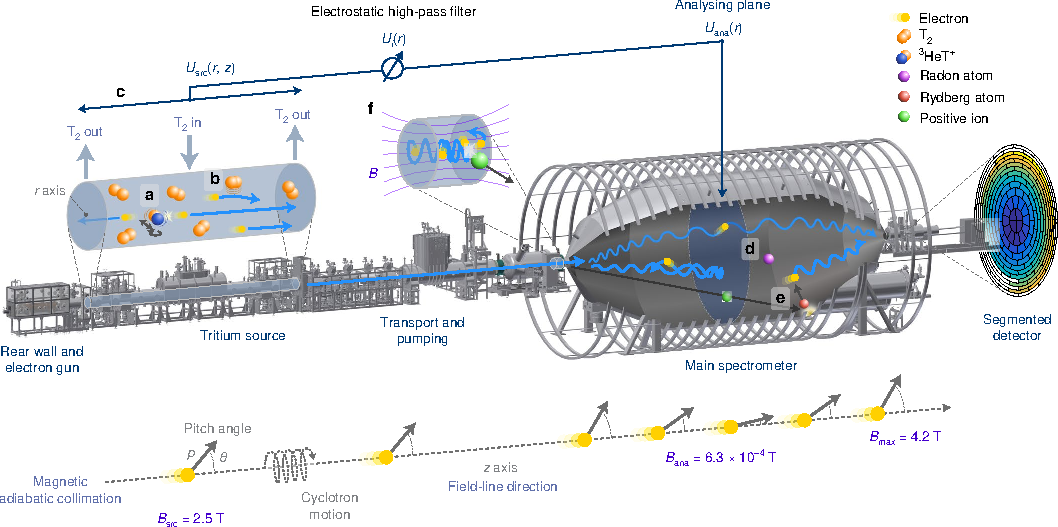
\includegraphics[width=0.92\textwidth]{figures/ch1/katrin.pdf}
  \caption{Illustration of the 70-m-long KATRIN beamline, also showing the transport of $\beta^-$ electrons and magnetic adiabatic 
collimation of their momenta in the spectrometer. View into the tritium source depicts three systematic effects:
molecular excitations during $\beta$ -decay (a), 
scattering of electrons off the gas molecules (b) and spatial distribution of the electric potential in the source (c). The view into the spectrometer 
illustrates the main background processes: radon decays (d), highly excited rydberg atoms 
due to $\alpha$-decays of $^{210}$Po (e) and positive ions created in a Penning trap between the two spectrometers 
(f). Image taken from  \cite{katrin2022direct}.}
  \label{fig:katrin}
\end{figure}
\subsubsection*{Project 8}

Traditional experiments using molecular tritium face limitations when neutrino masses approach $\sim$0.1 eV
due to broadening caused by internal molecular motion. To overcome these problems and achieve a hypotetical sensitivity
of 40 meV, the Project 8 Collaboration developed a novel technique called cyclotron radiation emission
spectroscopy (CRES) \cite{P8esfahani2017determining}. CRES utilizes the cyclotron emission from electrons or positrons
spiraling in a strong magnetic field to
determine their energies. This technique allows for incredibly precise measurements and is relatively immune to background interference, making it ideal for studying beta decay electrons.
The core of the CRES apparatus is a cryogenic gas cell, where electrons produced in radioactive decay are magnetically
trapped while emitting cyclotron radiation. The cell is placed in a superconducting magnet, generating an axial magnetic
field that confines electrons radially, while additional coils provide magnetic trap potentials to confine the electrons axially.

After demonstrating the feasibility of CRES on single electrons emitted from $^{83m}$Kr in the first phase of the experiment,
this technique was applied to perform the first spectrum measurement of molecular tritium beta decay near the
end-point region. This enabled the first neutrino mass limit using CRES, with a result of $m_{\overline{\nu}_{e}} < 155$ eV, concluding the
second phase. Moreover, the experiment achieved a stringent upper limit on backgrounds ($\le 3 \times 10^{-10}$ counts
eV$^{-1}$ s$^{-1}$) by characterizing and rejecting radiofrequency noise fluctuations, enabling a zero-background measurement. The objective of phase III is to demonstrate the ability to make CRES measurements in free space and produce and trap atomic tritium. The final phase aims to use atomic tritium to measure the neutrino mass with a sensitivity of 40 meV.
\begin{figure}[t]
\begin{subfigure}[b]{0.5\linewidth}
    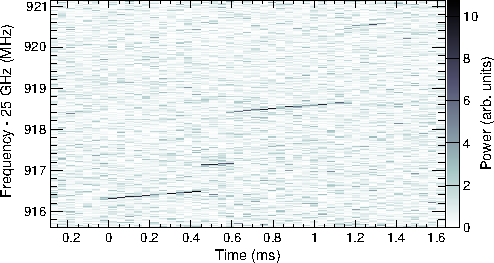
\includegraphics[width=\linewidth]{figures/ch1/p8electron.pdf}
    \caption{}
  \end{subfigure}
\hfill
\begin{subfigure}[b]{0.45\linewidth}
    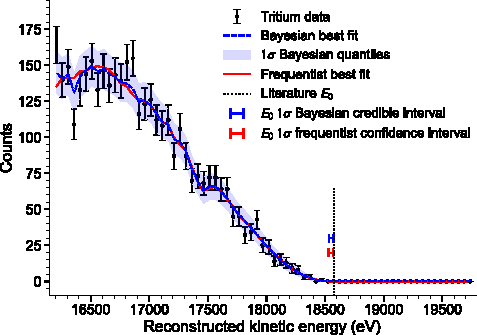
\includegraphics[width=\linewidth]{figures/ch1/p8V2.pdf}
    \caption{}
  \end{subfigure}
  \caption{Spectrogram of the first CRES event detected from a
tritium beta decay electron (a). Latest results of the project8 collaboration showing frequentist and bayesian fits of
the spectrum endpoint (b). Images taken from  \cite{P8esfahani2023tritium}. }
\label{fig:p8}
\end{figure}


\subsubsection*{Calorimetric experiments}
By embedding the radioactive source in the detector, calorimetric experiments measure all the energy of the decay,
excluding that carried away by the neutrino. This approach
minimizes the systematics due to source-related effects that are characteristic of spectrometric experiments. However, it comes
with the limitation that the entire energy spectrum is acquired, which imposes constraints on the source intensity in
order to limit the pile-up.
Pile-up events occur when multiple decays take place within a time interval shorter than the detector's time resolution
and are recorded as a single decay with summed energy.
The key component of these experiments is the microcalorimeter, a thermal detector that measures energy deposition
through heat conversion. When energy $E$ is deposited in the detector, it causes a temperature increase $\Delta T$,
which is proportional to $E/C$, where $C$ is the heat capacity of the detector. 

The thermodinamic limit defines how much
the measured energy fluctuates due to heat exchange with a thermal bath of temperature $T$:

\begin{equation}
  \Delta E \propto \sqrt{k_b T^2 C}
\end{equation}
Because of this, Low Temperature Detectors (LTDs) with small $C$ are employed in these experiments to minimize the thermal noise and achieve the best energy resolution possible.
Two completed experiments following this calorimetric approach used the beta decay of $^{187}$Re as their source. Known
as MANU and MIBETA  \cite{MANU} \cite{MIBETA}, they employed metallic and dielectric rhenium absorbers, respectively, to set limits of
$m_{\nu_{e}} < 19$ eV and $m_{\nu_{e}} < 15$ eV at the end of their measurement campaigns. However, these experiments
encountered challenges due to unexpected behaviors of metallic rhenium absorbers, including the Beta Environmental Fine
Structure (BEFS) \cite{koonin1991environmental} phenomenon, which rendered $^{187}$Re unsuitable for larger-scale experiments.

In recent years, significant interest has emerged in the use of $^{163}$Ho for estimating neutrino masses, which decays
via Electron Capture on an excited state of $^{163}$Dy. This isotope
possesses a lower $Q = 2833 \pm 30$ (stat) $\pm$ 15 (syst) eV compared to $^3$H and a shorter half-life
$T_{1/2} = 4570$ y than $^{187}$Re. 
A shorter half-life allows embedding smaller quantities of the isotope in the detectors, reducing the impact on their heat
capacity and thus preserving energy resolution.
The relatively short half-life and low Q value of $^{163}$Ho also allow for the use of a small absorbing volume, resulting in excellent energy resolution compared to other detectors in this energy range.
While other isotopes with lower Q values have been proposed, they often have extremely long half-lives, making
calorimetric experiments challenging or unfeasible in practice.

Among various proposed methods for measuring the neutrino mass with $^{163}$Ho, the calorimetric de-excitation spectrum
end-point measurement has shown to be the most promising.
Two collaborations, ECHo \cite{echofirst} and HOLMES \cite{alpert2015holmes}, are currently developing large-array experiments using Magnetic Metallic
Calorimeters (MMCs) and Transition Edge Sensors (TESs), respectively. The ECHO
collaboration has performed its first measurement campaign, reaching a limit of $m_{\nu_{e}}<150$eV at
90\% CL  \cite{velte2019high}.

In summary, a calorimetric experiment aiming for high sensitivity in neutrino mass determination has two primary
requirements: exceptional energy resolution and a substantial number of recorded events, which must be balanced with the
occurrence of pile-up events. For the Holmes experiment, Transition Edge Sensors (TESs) have been selected as the most
suitable detectors to satisfy these requirements. Their intrinsic energy resolution is exceptionally high, with resolving powers $\Delta E / E$
exceeding $10^3$ for single photons or electrons. This resolution can be preserved even when measuring arrays of
many calorimeters in a multiplexed setup, which allows accumulating the needed statistics and maintaining a fast signal
response.
\subsection{EC decay of $^{163}Ho$}

In the process of electron capture (EC) decay, an unstable nucleus captures an atomic electron, resulting in the production of a neutron, the emission of a neutrino, and the release of internal bremsstrahlung radiation. This process also leaves the daughter atom in an excited state, and subsequent emissions of X-rays and Auger electrons occur as the electron shell's vacancy is filled. In cases where the nuclide remains in an excited energy state, gamma radiation may be emitted. 

The EC decay of $^{163}$Ho can be represented as:


\begin{figure}[t]
  \begin{minipage}{0.43\linewidth}
    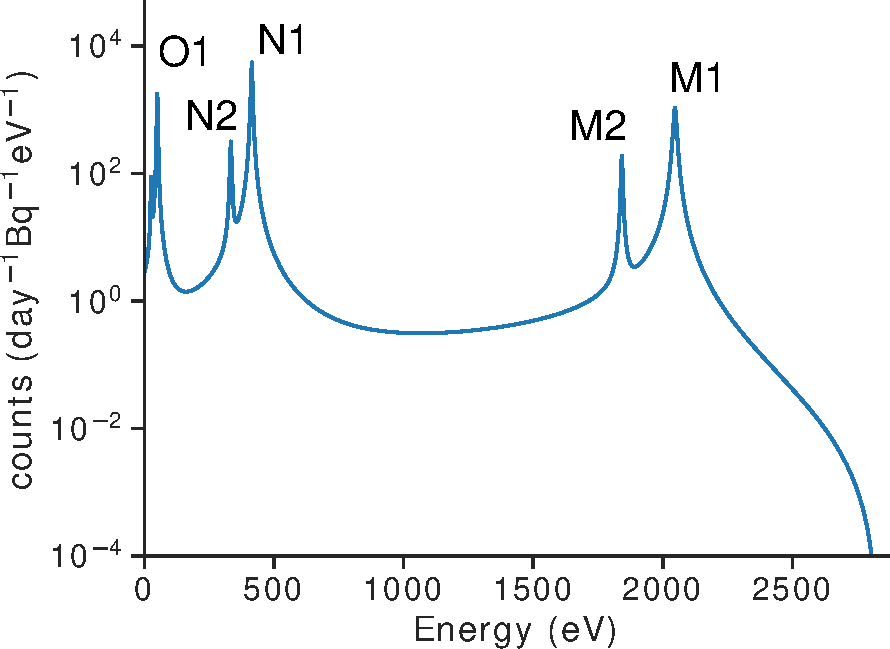
\includegraphics[width=\linewidth]{figures/ch1/Ho.pdf}
  \end{minipage}
  \hfill
  \begin{minipage}{0.58\linewidth}
      \centering
      \begin{tabular}{|c|c|c|c|c|}
        \hline
        Name & Orbital & \(E_H\) (eV) & \(\Gamma_H\) (eV) & $I_H$ \\
        \hline
        M1 & 3s & 2047 & 13.2 & 1 \\
        M2 & 3p$_{1 / 2}$ & 1842 & 6.0 & 0.0526 \\
        N1 & 4s & 414.2 & 5.4 & 0.2329 \\
        N2 & 4p & 333.5 & 5.3 & 0.0119 \\
        O1 & 5s & 49.9 & 3.0 & 0.0345 \\
        O2 & 5p$_{1 / 2}$ & 26.3 & 3.0 & 0.0015 \\
        \hline
    \end{tabular}
  \end{minipage}
\caption{first-order calorimetric spectrum of the $^{163}$Ho electronic capture decay, with $Q=2833$eV. The table shows
the names, corresponding electronic orbitals and parameters of the Lorentzian peaks.}
\label{fig:Hofirstorder}
\end{figure}
\begin{equation}
  ^{163}\text{Ho} + e^- \rightarrow ^{163}\text{Dy}_H + \nu_e \rightarrow ^{163}\text{Dy} + E_c
\end{equation}
Where $H$ labels the shell from which the electron has been captured, and $E_c$ represents all the energy of the decay
measured in a calorimetric experiment, which only excludes that of the neutrino. In the specific case of the EC decay of $^{163}
$Ho, there is no gamma emission, and the Dy atoms primarily decay through Auger processes rather
than X-rays. Therefore:
\begin{equation}
  E_c = \text{nuclear recoil} + \text{inner bremsstrahlung} + \text{Auger electrons} + \text{X-rays}
\end{equation}
Unlike beta decay, in EC decay the energy spectrum of the resulting neutrinos is similar to that of a two-body decay,
with the neutrino having an energy approximately equal to \(Q - E_H\), where \(E_H\) represents the binding energy of an
electronic
shell. The
complex structure of $^{163}$Ho poses challenges in predicting the shape of the calorimetric EC spectrum, and a
comprehensive description of its features still requries to be validated with extensive experimental data. At the first-order, the calorimetric spectrum consists of several Lorentzian-shaped peaks with energy \(E_H\) and natural width \(\Gamma_H\):

\begin{equation}\label{eq:hofirstorder}
\frac{dN_{EC}}{dE_c} \propto (Q - E_c)\sqrt{(Q - E_c)^2 - m_{\nu_e}^2}
\sum_H I_H\frac{\Gamma_H/2\pi}{(E_c - E_H)^2 + \Gamma_H^2/4}
\end{equation}

In this equation, \(I_H=|\phi_H(0)|^2 n_H B_{H}\) represents the intensity of each peak, where \(\phi(0)\) is the
wavefunction of the captured electron at the origin, \(n_H\) is the electron occupancy, and \(B_H\) is a corrective
factor accounting for atomic overlap and exchange. For $^{163}$Ho, the first-order spectrum consists of six main
Breit-Wigner peaks (M1, M2, N1, N2, O1 and O2). Their predicted parameters and the spectrum are shown in Fig
\ref{fig:Hofirstorder}.
As with beta decay, the endpoint region is the most sensitive to the neutrino mass, and the true energy spectrum should be
a coherent sum of three spectra with different endpoints corresponding to the three neutrino mass states, reducing to a
single spectrum with endpoint $Q-m_{\nu_{e}}$ if the energy resolution $\Delta E$ is greater than the magnitude of the neutrino mass.
However, the EC calorimetric measurement offers an advantage over beta decay: an enhanced count rate near the endpoint due to the proximity of the last atomic resonance.

\begin{figure}[t]
  \centering
  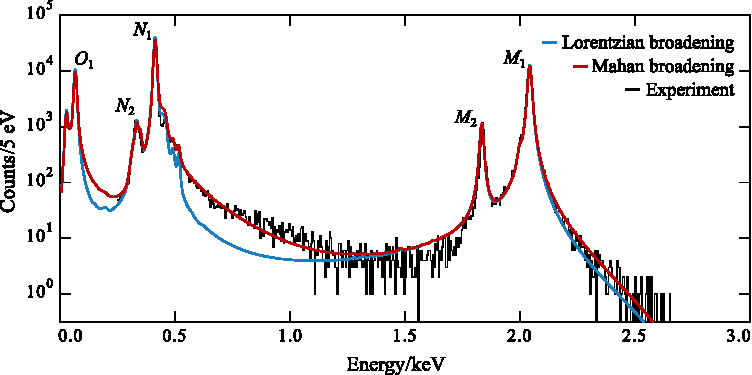
\includegraphics[width=0.75\textwidth]{figures/ch1/mahan.pdf}
  \caption{$^{163}$Ho nuclear decay spectrum measured by the Echo collaboration compared to ab initio theory broadened
  using a Lorentzian line-shape (blue) and Mahan line-shape (red). Image taken from  \cite{velte2019high}.}
  \label{fig:mahan}
\end{figure}


A more precise calculation of the spectrum requires considering second-order processes, which involve more electrons in the
decay. For example, when a second electron is promoted to another orbital, creating additional peaks, the phenomenon is
called "shake-up." If the electron escapes the atom and goes into the continuum spectrum, it is denoted as "shake-off."
The shake-off results in a broad and continuous alteration of the first-order spectrum, potentially enhancing the
statistics near the endpoint. Third and higher order processes are predicted to provide negligible
contributions \cite{thirdorder}.

More comprehensive descriptions, such as ab initio calculations, provide the best theoretical predictions available \cite{brass2018ab}. These methods reveal features beyond
the seven peaks, including shake-up and shake-off, asymmetric peak broadening, and energy shifts. The predicted
spectrum shows good but not perfect agreement with experimental data from the ECHO collaboration \cite{velte2019high}, as
shown in Figure \ref{fig:mahan}. The asymmetries appear to be mostly consistent with a Mahan broadening of the Breit-Wigner peaks, parametrized with an electron energy cutoff \(\xi\) and asymmetry \(\alpha\):

\begin{equation}
M_H(E) = \int_{0}^{\infty} L_H(E_c - E') \frac{1}{\xi \Gamma(\alpha)} \frac{e^{-E'/\xi}}{(E'/\xi)^{1-\alpha}} dE'
\end{equation}
Where \(L_H(E_c)\) denotes the Lorentzian function describing a peak in the first-order approximation. 
To allow for comparison between theoretical predictions and data, the experimental spectrum \(S(E_c)\) is obtained from
the theoretical spectrum \(S_{EC}(E_c)\) by considering pile-up events, the background, and the energy resolution of the
experiment. The pile-up spectrum is approximated as the convolution of the single spectrum with itself, multiplied by the fraction of unresolved pile-up events \(f_{pp}\). The experimental spectrum is expressed as:

\begin{equation}
S(E_c) = \left[ (1-f_{pp}-f_{bkg})S_{EC}(E_c) + f_{pp} S_{EC}(E_c) * S_{EC}(E_c) + f_{bkg}B(E_c) \right] * R_{\Delta E}(E_c)
\end{equation}

Here, \(B(E_c)\) is the background spectrum, and \(R_{\Delta E}(E_c)\) is the energy response of the detector, usually
a Gaussian, corresponding to
an energy resolution \(\Delta E\).
\section{The Holmes detector}
\subsection{Transition Edge Sensors}\label{sec:TES}

The detectors used in the Holmes experiment consist of three essential components: an absorber doped with $^{163}$Ho to convert radiation
energy into heat, a Transition Edge Sensor (TES) thermometer to translate heat into a measurable signal, and an
insulating structure to confine the energy for precise measurement before restoring the idle temperature after an event. Among Low Temperature Detectors, superconducting TESs offer high resolution and efficient multiplexing readout techniques.
A TES serves as a sensitive thermometer by operating within the narrow temperature range of the transition between the
superconductive and resistive states of a metal \cite{irwin2005TESreview}. When energy is deposited in an absorber
thermally linked
to a TES, the resulting temperature change causes a resistance variation in the
TES. If a constant voltage bias is applied, this change of resistance leads to a measurable drop in the current flowing
through the TES. Consequently, a
change in energy corresponds to an observed change in current.% The working point of a TES is usually expressed as a percentage of the normal resistivity $R_n$ of the metal, indicating at which point in the transition it has been biased.

The sensitivity of TESs arises from the sharpness of the superconductive-to-normal metal transition. However, the
complex physics of this phenomenon makes predicting the detector's behavior challenging. The resistance of a TES mainly
depends on temperature and current, denoted as $R(I, T)$, and is also weakly dependent on the local magnetic field, which can typically be neglected.
A simplified description of a voltage-biased TES can be represented by an electrothermal circuit, as shown in Figure
\ref{fig:TEScircuit}. The voltage bias is achieved by applying a constant current to a small shunt
resistance $R_{sh}$ parallel to the TES and to an inductance $L$, which corresponds to a Thevenin equivalent circuit with
constant voltage $V$ and load resistance $R_{L}=R_{sh}$. The TES, modeled as a variable resistor $R_{TES}$, is coupled to an
absorber with heat capacity $C$, exchanging heat with the thermal bath through a heat conductance $G$. The evolution of
this system is determined by two differential equations:

\begin{eqnarray}
  C \frac{dT}{dt} = -P_{\text{bath}} + P_J + P \\ \label{eq:et1}
  L \frac{dI}{dt} = V - IR_{sh} - IR_{\text{tes}} \label{eq:et2}
\end{eqnarray}

These equations couple the electrical and thermal responses through the nonlinear quantities $R_{TES} = R_{TES}(I, T)$
and $P_J = R_{TES}I^2$. Moreover, they show that operating a TES in the voltage-biased regime, where $R_{sh} \ll R_{TES}
$, offers advantages. When energy is deposited in the absorber, causing an increase in temperature and TES resistance,
the reduced current flow decreases the Joule power dissipation in the TES, restoring the initial temperature after a
short transient. This effect, known as negative electrothermal feedback (ETF), stabilizes the TES's operational state. 
\begin{figure}[t]
    \begin{subfigure}[b]{0.5\linewidth}
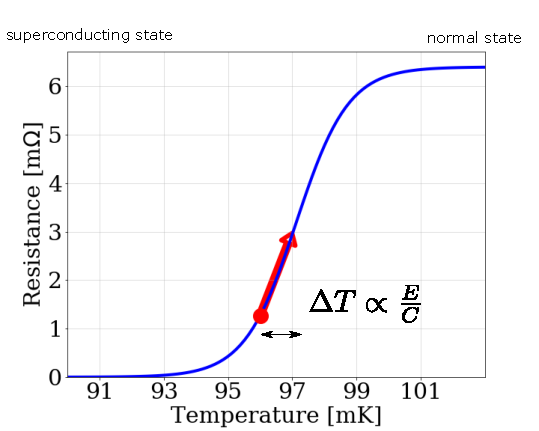
\includegraphics[width=\linewidth]{figures/ch1/TEStheory.pdf}
\caption{}
\end{subfigure}
\hspace{0.5cm}
\begin{subfigure}[b]{0.35\linewidth}
    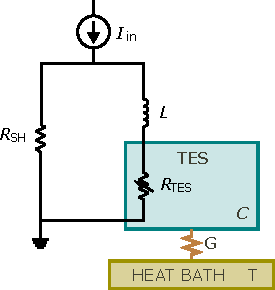
\includegraphics[width=\linewidth]{figures/ch1/TEScircuit.pdf}
\caption{}
\end{subfigure}
\caption{Operating principle of a Transition Edge Sensor (a). Electrothermal circuit diagram for a voltage
biased TES (b).} 
\label{fig:TEScircuit}
\end{figure}

The response differential equations can be solved in the small signal approximation by linearizing the resistance with a
first-order expansion, assuming that its change due to absorbed energy is small compared to
the at-rest TES state $R_0(I_0, T_0)$. Two logarithmic derivatives, denoted as $\alpha$ and $\beta$, define the sensitivity to
temperature and current changes:

\begin{equation}
\alpha = \frac{\partial \log R}{\partial \log T}\Bigg|_{I_0=T_0,R_0} \quad  \quad \beta = \frac{\partial \log R}{\partial \log I}\Bigg|_{T_0=I_0,R_0}
\end{equation}

The resistance and dissipated power can then be linearized for small deviations $\delta T = T - T_0$ and $\delta I =
I - I_0$:

\begin{eqnarray}
R(T, I) \sim R_0 + \alpha R_0 \delta T + \beta R_0 \delta I\\
P_J \equiv I^2R \sim P_{J0} + 2I_0R_0\delta I + \alpha P_{J0}\delta T + \beta P_{J0}\delta I
\end{eqnarray}

These approximations allow deriving analytical solutions for the differential equations \ref{eq:et1}. While the small signal approximation does not precisely predict the detector's response, it provides valuable information about signal parameters and noise spectrum, as well as expected energy resolution.
The noise spectrum is characterized by three main sources: the Johnson noise of the TES resistance, that of the load or
shunt resistor, and the thermal fluctuation noise. Observed additional noise has been linked to the thermal circuit
configuration, but some unexplained sources still persist.
For small signals and strong negative ETF, it can be shown that the TES energy resolution is proportional to:
\begin{equation}
  \Delta E\propto \sqrt{{4k_B T^2 C}{\sqrt{\frac{1+2\beta}{\alpha}}}}
\end{equation}
This relationship shows that optimal operation of the TES requires proper combination of temperature, current and bias
to maintain low current sensitivity $\beta$ and high temperature sensitivity $\alpha$ \cite{zhou2020towards}. 

A more comprehensive treatment of the TES response in the large signal regime requires an understanding of the mechanisms
underlying the superconducting transition. For larger TES devices, such as those used in the Holmes detector,
experimental observations are consistent with a two-fluid model featuring Phase Slip Lines (PSLs) \cite{PSLcenters}. In the context of
superconductivity, the macroscopic wave function of the Cooper pairs $\psi(r) = |\psi(r)|e^{i\phi(r)}$ serves as the
order parameter. This order parameter exhibits amplitude and phase coherence, which disappear at the critical
temperature or current, marking the transition to the normal phase.
\begin{figure}[t]
\begin{subfigure}[b]{0.4\linewidth}
    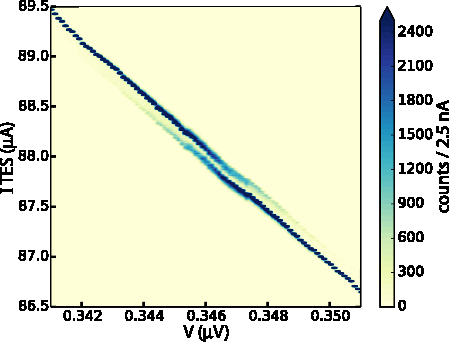
\includegraphics[width=\linewidth]{figures/ch1/PSL1.pdf}
    \caption{}
  \end{subfigure}
\hfill
\begin{subfigure}[b]{0.5\linewidth}
    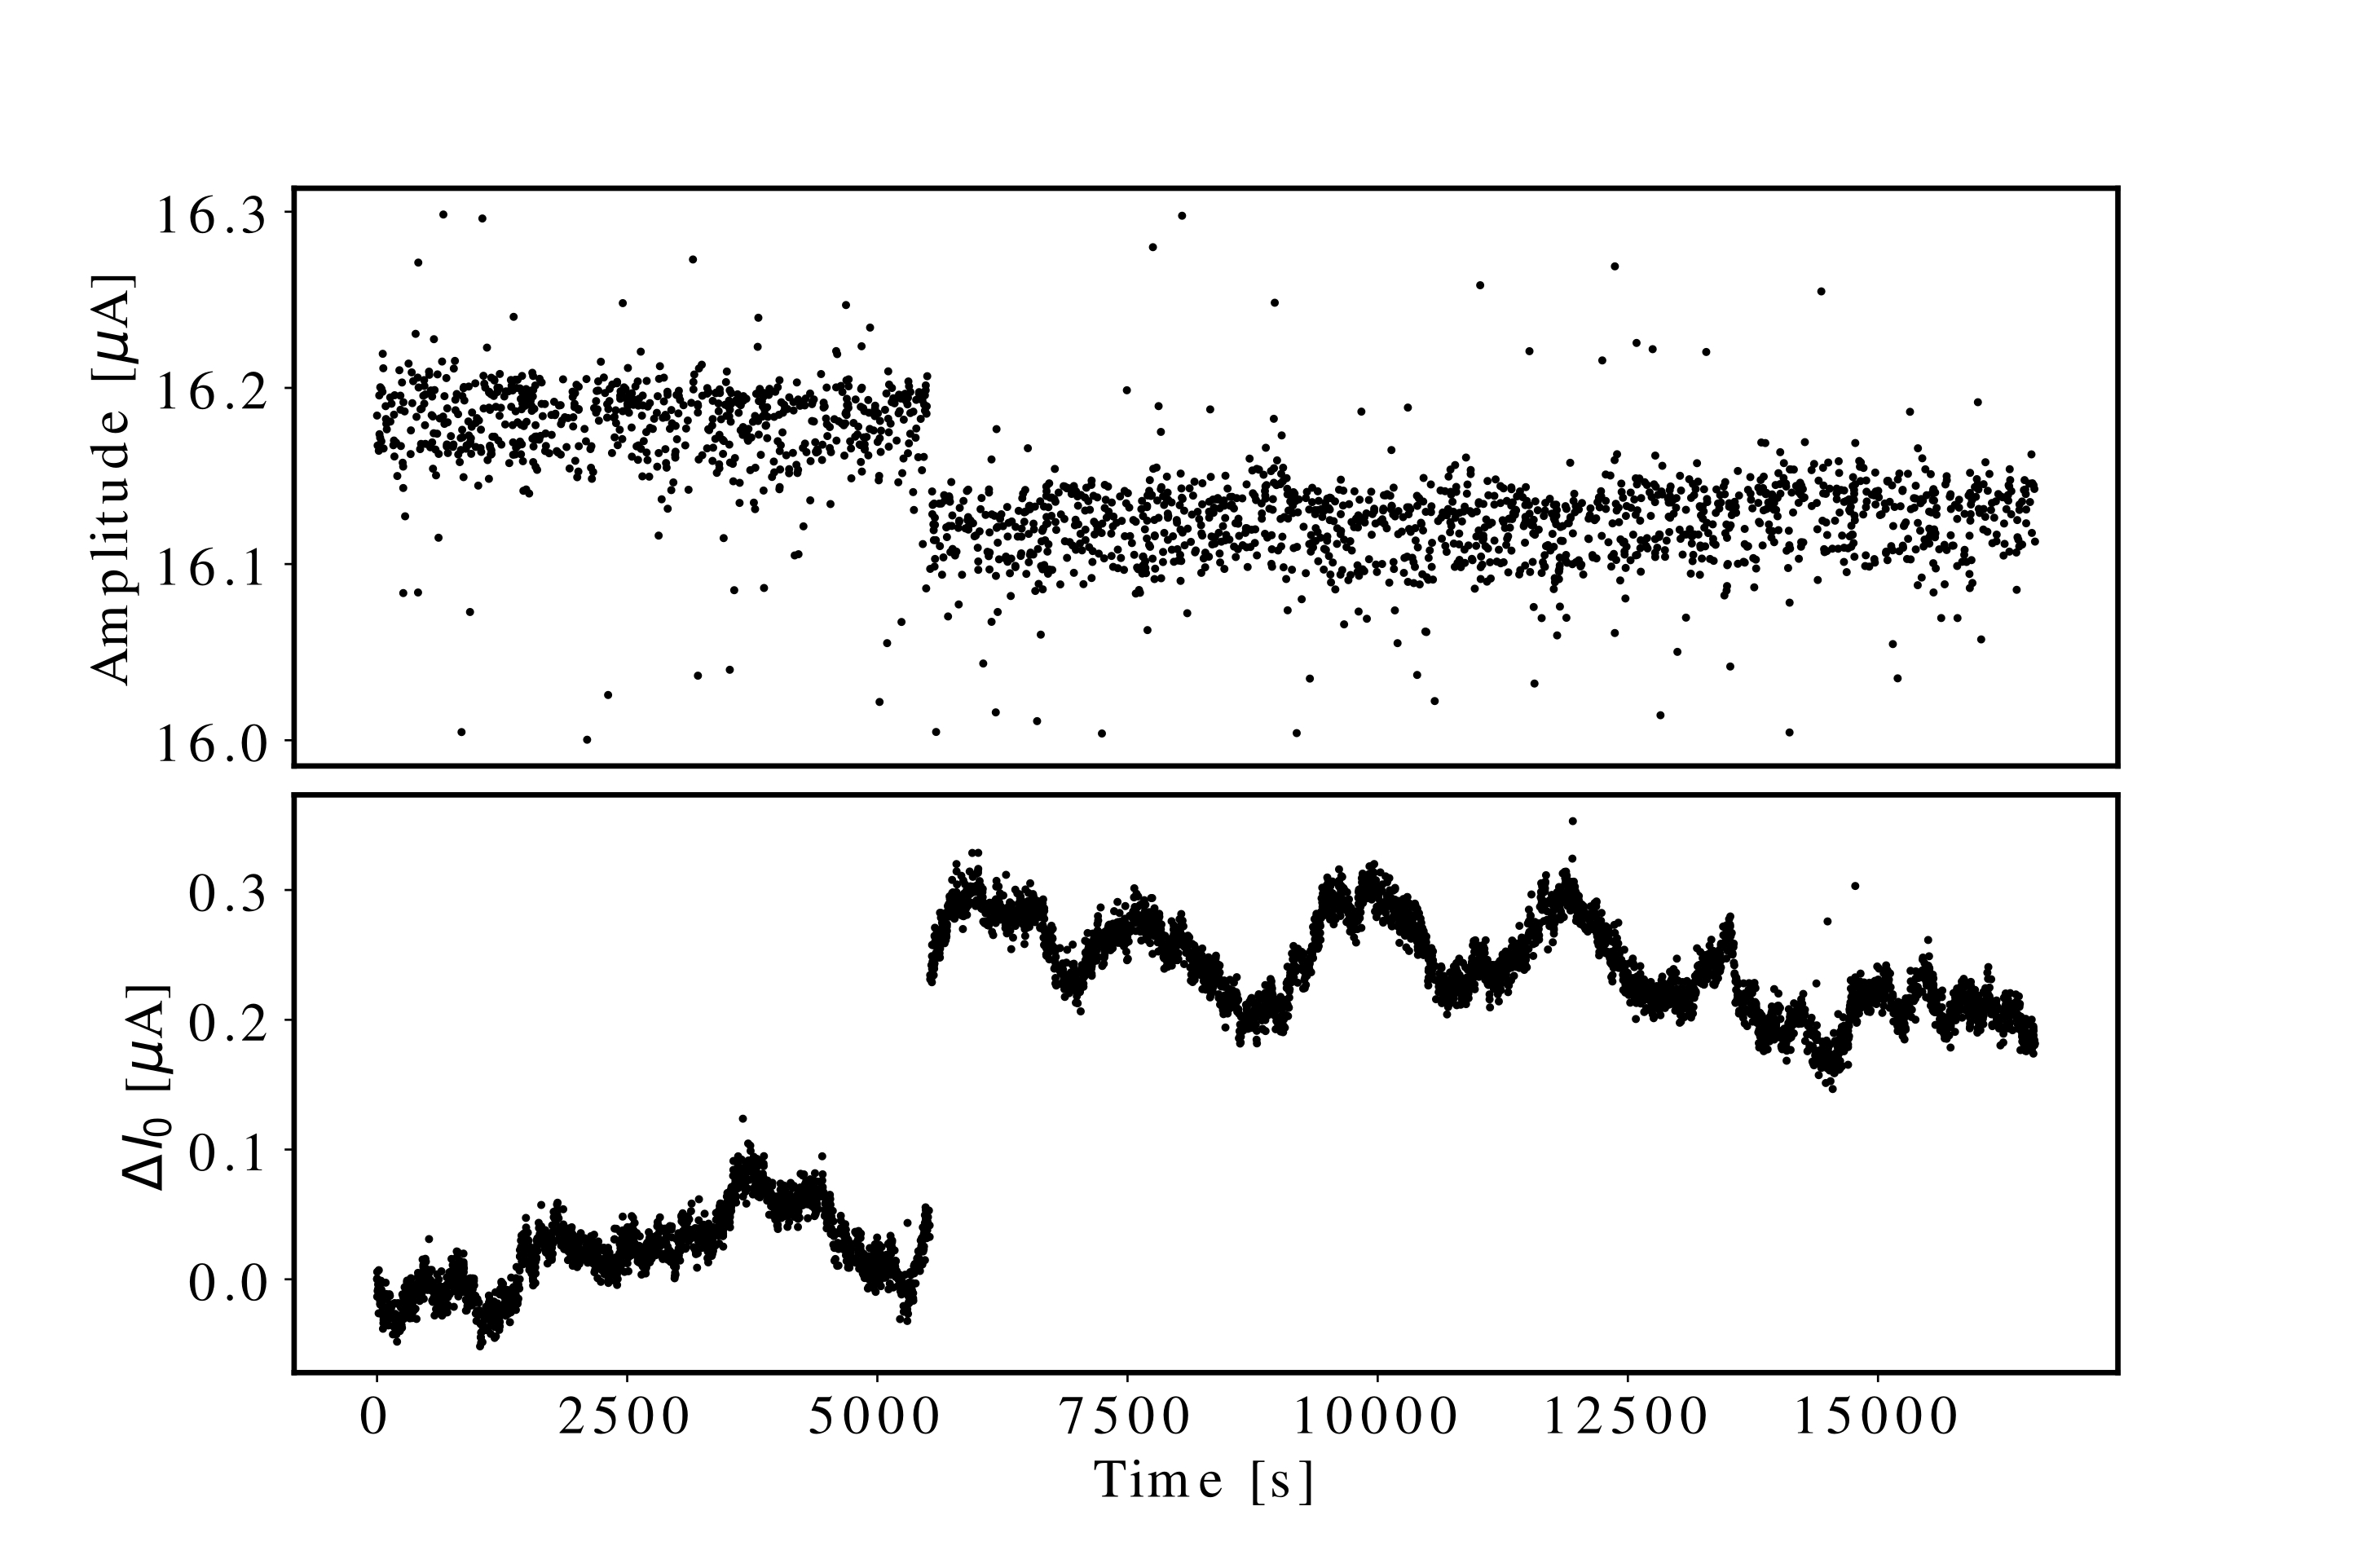
\includegraphics[width=\linewidth]{figures/ch1/PLS2.jpg}
    \caption{}
  \end{subfigure}
  \caption{Measured IV characteristic of a TES. For each bias voltage, 130000
    measurements of the current are histogrammed (a). Image taken from  \cite{PSL}. Sudden variation in the idle current of the TES
used by the Holmes experiment, resulting in different signal amplitude for events originating from an approximally
monochromatic X-ray source (b). Image taken from  \cite{borghesi2022toward}}
\label{fig:PSL}
\end{figure}
This transition does not occur uniformly across the entirety of the superconducting material. Instead, phase slips
manifest as localized regions within the superconductor where the current surpasses its critical value and becomes
partially carried by quasi-particles, thereby generating a potential difference. Along the boundaries of these phase
slips, two supercurrents with distinct order parameters emerge. In filamentary superconductors, phase slips correspond
to nucleation centers, whereas in two-dimensional films, they appear as lines perpendicular to the direction of current
flow. For a given voltage drop across the TES, different numbers of phase slip lines $n_{PSL}$ can be present, resulting
in multiple potential values of observed current. This phenomenon leads to bimodal structures in the current-voltage (IV) curve.
These predictions can be experimentally verified  \cite{PSL}, as illustrated in Figure \ref{fig:PSL}.
Furthermore, the model provides insight into another phenomenon observed in the Holmes detectors, where the signal
amplitude of the TES for events with approximately the same energy abruptly changes and remains in this altered state
for several minutes. This behavior may be attributed to the fact that, on occasion, the detector settles into a stable
state characterized by a different number of PSLs compared to the initial state before the event \cite{borghesi2022toward}.



\subsection{Microwave Multiplexing readout}\label{sec:muMUX}
Since a substantial
number of microcalorimeters is needed for a meaningful measurement of $m_{\nu_{e}}$, the readout system must provide a
high multiplexing factor while maintaining a fast signal response to limit pile-up events. Multiplexing refers to the ability to read
multiple detectors with a single electrical connection within the cryostat.
Its primary objective is to shift the complexity of the experimental setup outside the cryostat to the warm stage. 
Without multiplexing, the number of wire
pairs required to operate all the TESs employed by Holmes would be unmanageably high, leading to excessive heat generation at the cryogenic stage.

In recent years, Microwave SQUID Multiplexing ($\mu$MUX) has emerged as a practical and consistent method for reading arrays
of microcalorimeters, satisfying the necessary requirements and outperforming other multiplexing techniques such as time
or frequency division multiplexing \cite{muMUX}.
The $\mu$MUX readout chip comprises a series of quarter-wave resonators, each coupled to an rf-SQUID (radio-frequency
Superconducting Quantum Interference Device), which is used to adjust their resonant frequencies. An rf-SQUID consists
of a superconducting loop interrupted by a single Josephson junction, a circuit element with no classical
equivalent consisting of two overlayed superconducting terminals separated by a thin insulator. The
response of a Josephson junction is determined by the tunneling of Cooper pairs through the barrier and can be described
as a nonlinear inductance dependent on the phase difference $\phi$ between the wavefunctions at the junction's sides:

\begin{equation}
L(\phi) = \frac{L_J}{\sin\phi}, \quad L_J= \frac{\hbar}{2eI_c}= \frac{\Phi_0}{2\pi I_c}
\end{equation}
Here, \(I_c\) represents the critical current of the superconductor and \(\Phi_0\) denotes the magnetic flux quantum.
When the self-inductance of an rf-SQUID \(L_S\) is less than that of the Josephson junction \(L_J\), the loop functions as an extremely sensitive magnetometer. The phase difference becomes proportional to the magnetic flux through the loop:

\begin{equation}
  \phi=\frac{2e}{\hbar}\int\left(\frac{d\Phi}{dt}\right)dt =2\pi\frac{\Phi}{\Phi_{0}}
\end{equation}
A variation in flux leads to a change in current and voltage drop across the junction, which depend on the phase and
its time derivative:
\begin{equation}
  \frac{2e V}{\hbar} = \frac{d\phi}{dt}, \quad I = I_c \sin\phi
  \label{eq:JJ}
\end{equation}
The rf-SQUID can be read by inductively coupling it to another circuit, the impedance of which is then dependent on variations
of the observed flux. In the case of the $\mu$MUX chip, each rf-SQUID is coupled to a resonator designed to
ring at a unique frequency. Many resonators are coupled to a common feedline, allowing for their
simultaneous readout by sending through
the feedline a combination of fixed gigahertz signals at the resonating frequencies. Changes in the flux applied to a SQUID result in changes of the corresponding resonator's impedance and resonant
frequency, which manifest as shifts in the phase and amplitude of the probe signal at the specific frequency.
The phase signals are larger than those in amplitude, and the latter are usually discarded.
In this way, rf-SQUIDs amplify the weak signal currents generated in a TES, while the resonators enable to differentiate each microcalorimeter using a distinct frequency.

In summary, an energy deposition in a voltage-biased TES results in a change in its resistance and current flow,
typically in the order of tens of microamperes. Through the TES circuit's
inductance, this current generates a magnetic flux that is read and amplified by an rf-SQUID, altering the resonant frequency of the corresponding resonator.
When the resonator is probed at a fixed frequency, this results in an observable signal, which is read as a phase difference in the circuit's response.

This setup is further complicated by the fact that the SQUID's response to changes in magnetic flux is periodic rather
than linear, as can be seen from Eq \ref{eq:JJ}. Therefore, a method called flux ramp
modulation is employed to linearize the SQUID's response \cite{mates2012flux}. Figure \ref{fig:multireadout} depicts the complete multiplexing and readout circuit for Holmes,
including voltage bias and flux modulation.
\begin{figure}[t]
  \centering
  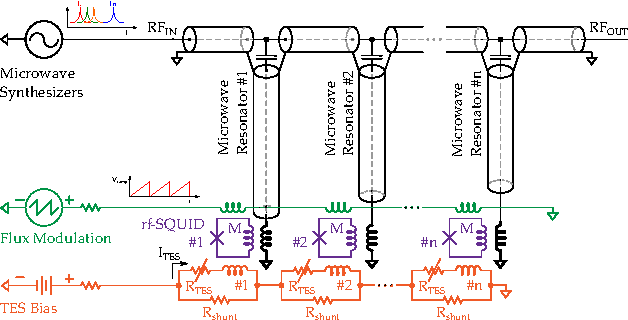
\includegraphics[width=0.8\textwidth]{figures/ch1/HOLMEScircuit.pdf}
  \caption{Circuit diagram of the multiplexing and readout scheme used by Holmes.}
  \label{fig:multireadout}
\end{figure}
In this modulation scheme, a common flux ramp signal is applied to all SQUIDs. The flux ramp is a sawtooth signal that resets at a frequency of \(f_{\text{ramp}}\) and has an amplitude set to induce integer multiples of flux quanta (\(n\Phi_0\)) in the SQUIDs, causing them to perform identical and periodic oscillations during each ramp cycle.
If the frequency of the applied ramp exceeds the maximum frequency content of any input signal, a change in the TES
current ad thus a variation of the SQUID input corresponds to a phase offset in the SQUID's ramp-induced oscillation.
This phase shift is directly proportional to the magnetic flux through the loop and can be measured using a Fourier
transform of the observed SQUID oscillation.
At each ramp cycle, the SQUID response $S(t)$ is sampled a certain number of times. Then, the phase offset is obtained
by performing a Fourier measurement between the samples:
\begin{equation}
I \propto \phi = \arctan\left(- \frac{\sum S(t) \sin(2\pi n\Phi_0 f_{\text{ramp}} t)}{\sum S(t) \cos(2\pi n\Phi_0 f_{\text{ramp}} t)}\right)  
\end{equation}
In this way, the TES signal is sampled with frequency $f_{ramp}$, once every ramp cycle.
This parameter must be chosen carefully to obtain an adequate number of samples during the rise time of the TES pulse,
typically around 10, while avoiding degradation of the detector's intrinsic energy resolution. The maximum sampling
frequency thus sets a limit on the speed of the detector response. 

The number of detectors that can be read simultaneously using this readout system, known as the multiplexing factor
\(N_{\text{det}}\), is limited by the total frequency range available, denoted as the bandwidth \(BW\):

\begin{equation}
N_{\text{det}} = \frac{BW}{f_{\text{ramp}} \cdot n\Phi_0 \cdot K \cdot 2} 
\end{equation}
Here, \(K\) is a "guard factor" proportional to the resonance spacing, designed to prevent crosstalk between adjacent
resonances characterized by width $BW_{\text{res}}$:

\begin{equation}
K = \frac{f_{\text{res}, n+1} - f_{\text{res}, n}}{BW_{\text{res}}}   
\end{equation}
Holmes employs the $\mu$mux17a, a 33-channel multiplexing chip developed and fabricated at the National Institute for
Standards and Technology (NIST, Boulder, CO, USA). It features a total bandwidth of \(BW = 550\) MHz, a resonance
bandwidth of approximately \(BW_{\text{res}} \approx 2\) MHz and resonance spacing of 14 MHz, corresponding to $K=7$.
With a ramp frequency of 500 kHz and two SQUID oscillations per cycle, this results in a multiplexing factor of approximately \(N_{\text{det}} \approx 39\).

\subsection{Detectors design and fabrication}\label{sec:fabrication}
Each TES in the Holmes detectors consists of a $125\times125\mu \text{m}^2$ metal bilayer composed of molybdenum
and copper, which suppresses the critical temperature of Mo from 920mK to 100mK. The bilayer features copper bars
oriented orthogonally to the current flow which have been shown to reduce excess electrical noise and allow to tune the
normal resistance $R_n$.
A gold absorber measuring 180 × 180 × 2 $\mu m^3$ is chosen to provide high stopping power, low heat capacity, and efficient
thermalization properties. The de-excitation products of Ho decay, such as Auger electrons and X-rays, undergo
relaxation through electron-electron and electron-phonon scattering interactions within a fraction of a nanosecond. It is
predicted that the chosen absorber thickness allows for a 99.99\% probability of stopping electrons and a 96.73\%
probability of stopping photons from the decay.
As the Au absorber is deposited atop a copper structure with a connecting bar to the TES, their temperature become closely coupled, ensuring thermal equilibrium between the two components.
The current design of the Holmes detector, shown in Fig \ref{fig:TES}, employs a sidecar geometry to mitigate the proximity effect between the
thermal sensors and the absorber, which could otherwise alter the resistance profile in the transition.


\begin{figure}[!b]
    \begin{subfigure}[b]{0.3\linewidth}
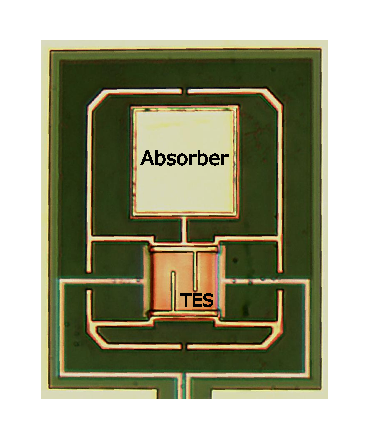
\includegraphics[width=\linewidth]{figures/ch1/TES.pdf}
\caption{}
\end{subfigure}
\hspace{1.5cm}
\begin{subfigure}[b]{0.55\linewidth}
    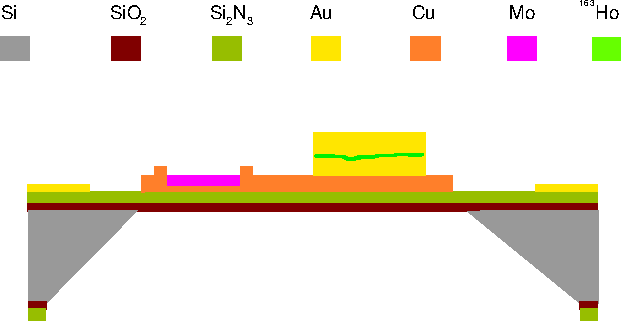
\includegraphics[width=\linewidth]{figures/ch1/TESdesign.pdf}
\caption{}
\end{subfigure}
\caption{Top view of a microcalorimeter used by the Holmes experiment, showing an absorber and TES suspended over a
thin Si$_2$N$_3$ membrane, which appears dark in the photo (a). Side view of the detector, illustrating the different
materials used in the current design (b). The figure is not to scale.} 
\label{fig:TES}
\end{figure}
Achieving thermal isolation of the detector is crucial for measuring all the energy released in an event and tailoring the signal time profile to match the readout
system's bandwidth and sampling frequency. The detectors used by Holmes are positioned on a suspended silicon nitride Si$_2$N$_3$
membrane, preventing the escape of hot phonons during the thermalization process. The
membrane's thickness is approximately 500 nm. 

Moreover, to minimize experimental dead-time, the heat dissipation from the perimeter of the detector to the thermal bath is enhanced with a thin copper trace around the detector. This has been demonstrated to
increase the thermal conductance while minimally affecting heat capacity, thus preserving energy resolution.
The detectors fabrication undergoes three phases: 
\begin{description}
  \item[Array fabrication at NIST:] After having produced the bare circuit for a 64 detectors array with standard techniques, a photoresist
    mask exposing only the absorbers is applied and the first $1\mu$m of gold is deposited over the photoresist.
  \item[Ho production and implantation:]
The necessary $^{163}$Ho must be synthesized through thermal neutron irradiation. Enriched $^{162}$Er$_2$O$_3$ powder
was irradiated at the ILL nuclear reactor in Grenoble, France, with the resulting $^{163}$Er decaying to $^{163}$Ho via electron capture. 
\begin{equation}
^{162}\text{Er}(n, \gamma)^{163}\text{Er} \rightarrow ^{163}\text{Ho} + \nu_e
\end{equation}
To ensure the purity of the obtained holmium, chemical purification processes were conducted at the Paul Scherrer
Institute, yielding approximately a total of 200 MBq of $^{163}$Ho.
A custom ion implanter housed in Genoa, which will be discussed in more detail in the next section, is used to
incorporate the $^{163}$Ho nuclei into the TES absorbers. The core component
of the implanter is a sputter ion source that generates argon plasma from thermoionic electrons. The plasma exctracts Ho ions from a
target, and the obtained ions are accelerated and collimated in a beam. Subsequently, a magnetic selector,
consisting of a dipole magnet, separates the $^{163}$Ho ions from other contaminants before projecting the beam onto the TES
array.  

\item[Array finalization in Milan:] The final $1\mu$m of gold is deposited over the implanted detectors with a system
    consisting of four Compact Microwave and Coaxial (COMIC) ion sources placed in a high
vacuum environment, denoted as the target chamber. Each COMIC source uses an electric field generated by antennas within a magnetic cylinder to ignite
an argon plasma, which is used to create four focused argon ion beams directed at ultra-pure gold targets, depositing
part of the sputtered gold on the detectors array. The excess gold is then removed with the lift-off of the
photoresist mask by dipping the array in acetone. 
Finally, the thin Si$_2$N$_3$ membranes over which the TES are suspended to achieve thermal isolation are exposed with a KOH
etching process. A potassium hydroxide solution is used to etch silicon, producing almost vertical
walls. The technique provides consistent results, and the etched areas exhibit good uniformity and quality.
\end{description}





\section{Experimental setup}\label{sec:setup}
\subsection{Detector holder and calibration sources}\label{sec:holder}

\begin{figure}[t]
    \begin{subfigure}[b]{0.68\linewidth}
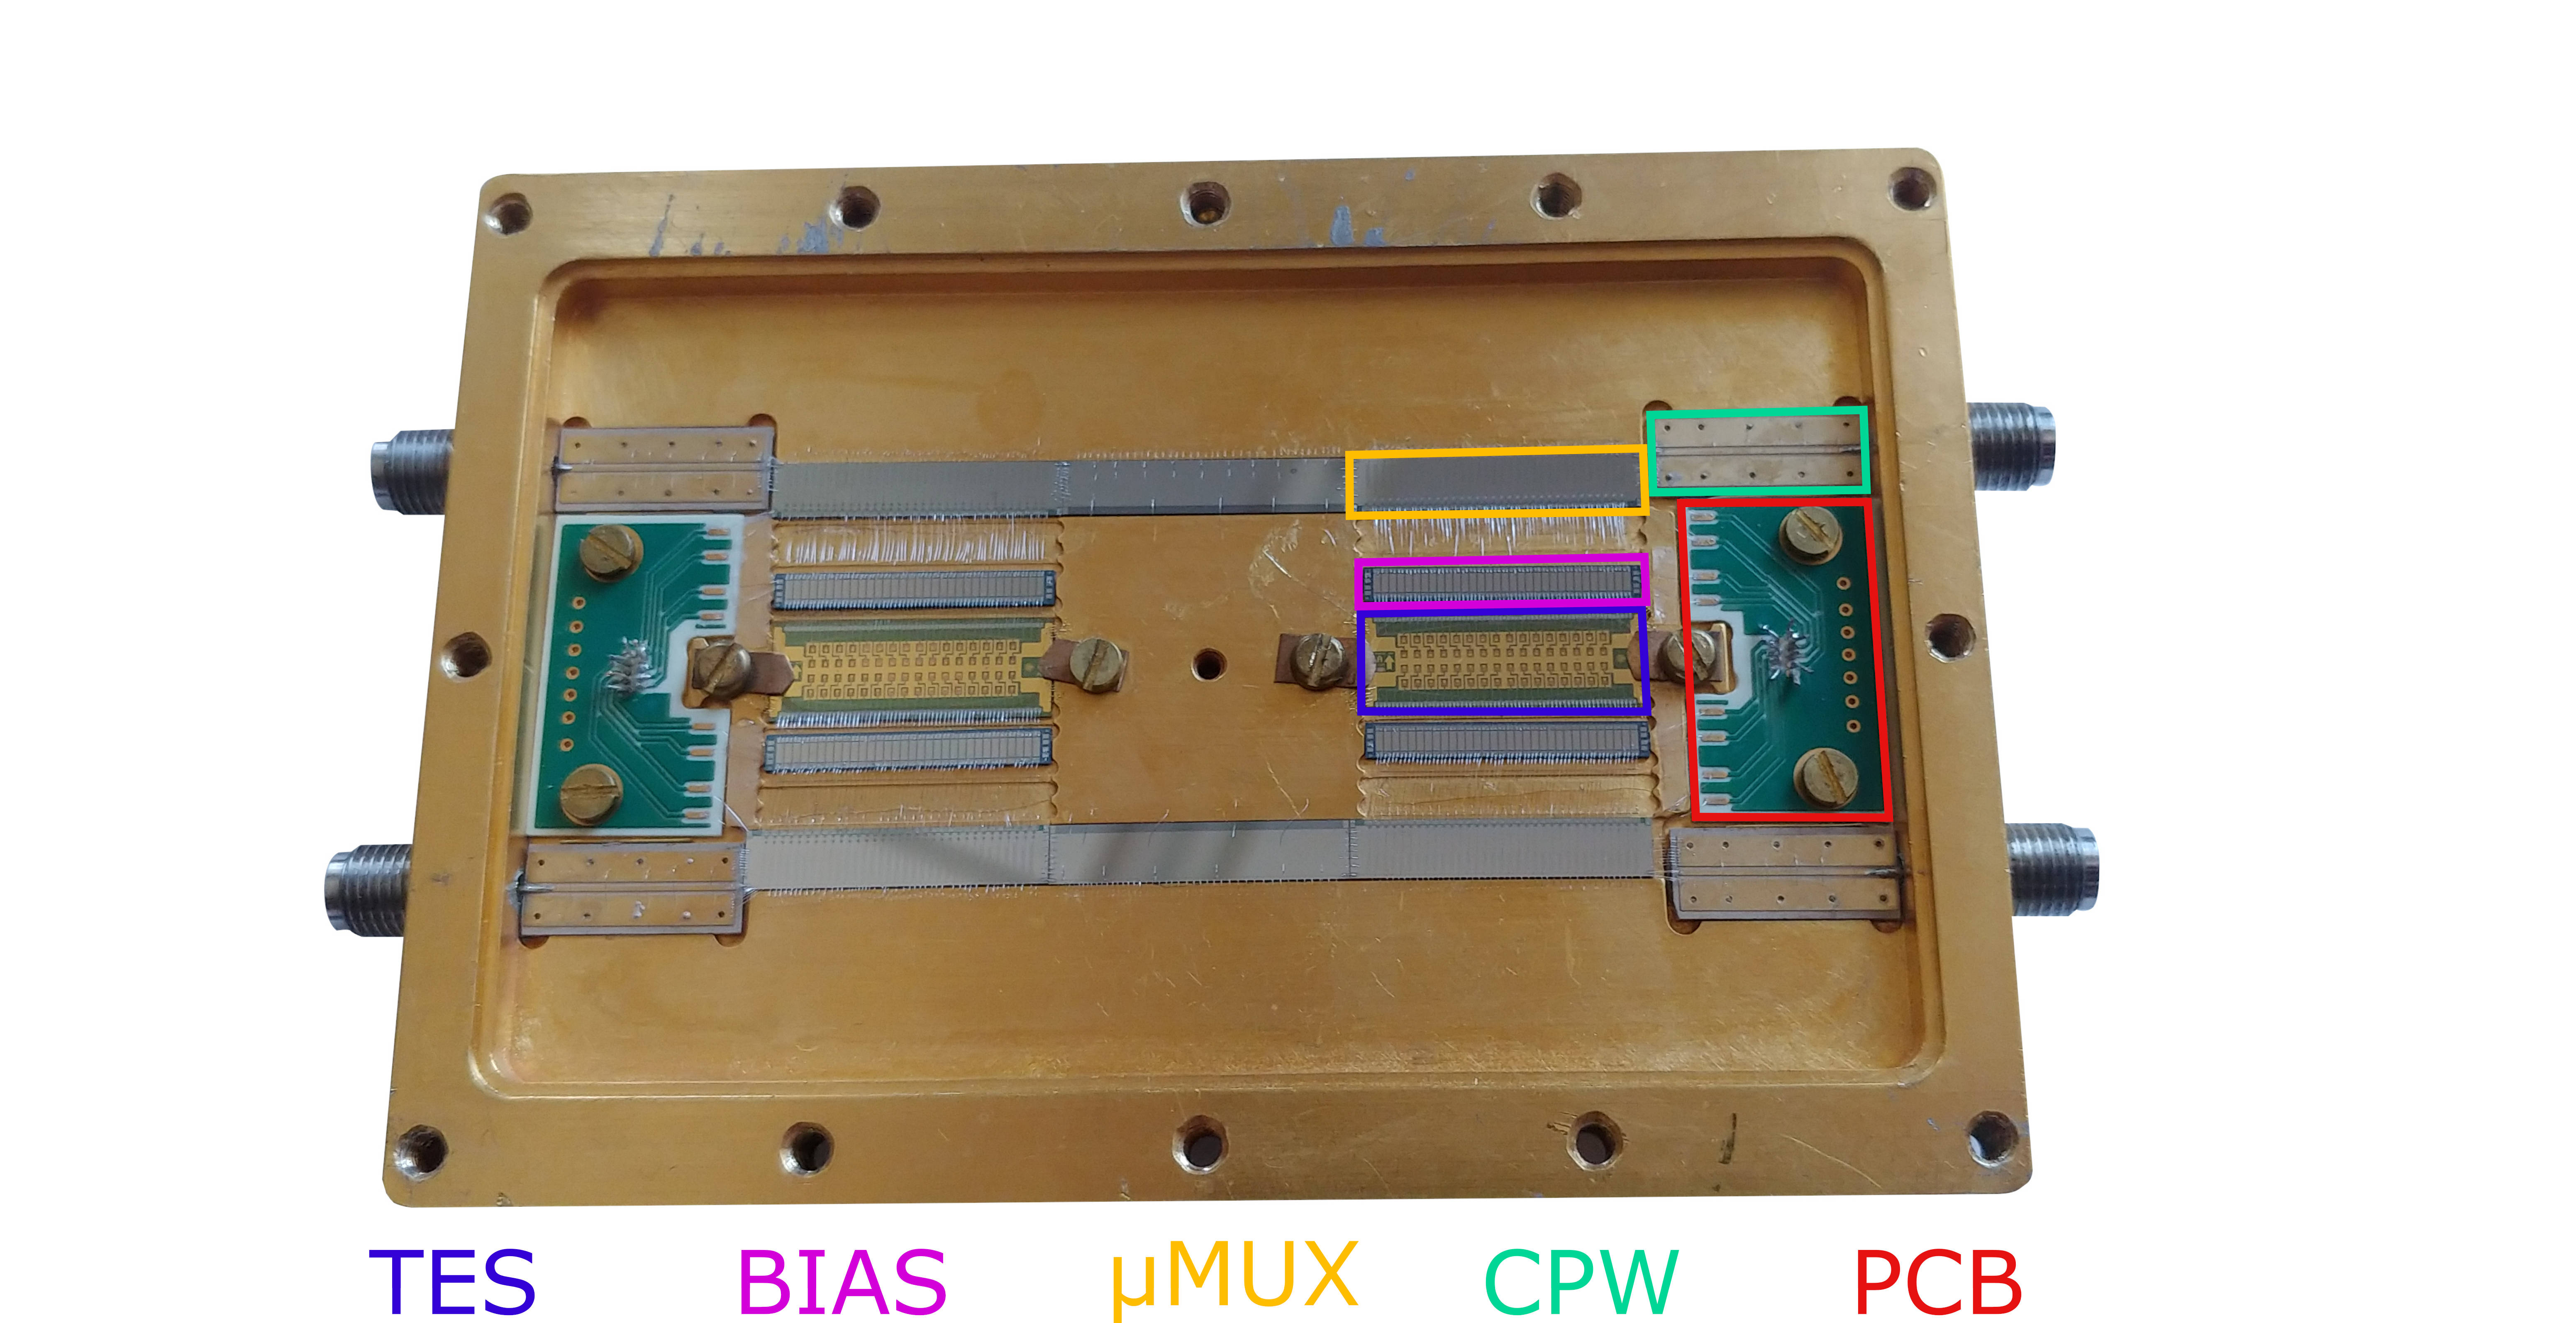
\includegraphics[width=\linewidth]{figures/ch1/holderfi.jpg}
\caption{}
\end{subfigure}
\begin{subfigure}[b]{0.3\linewidth}
    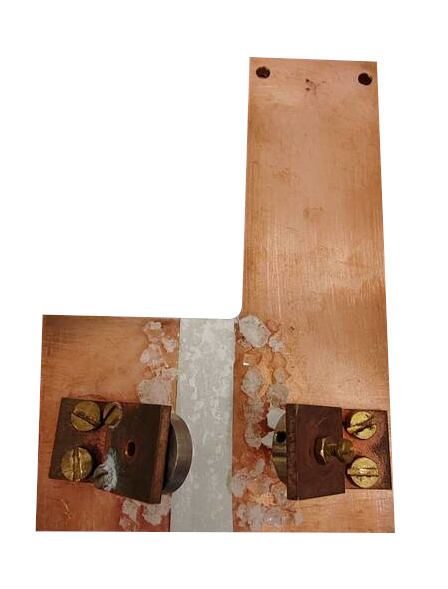
\includegraphics[width=0.9\linewidth]{figures/ch1/calcrop.jpg}
\caption{}
\end{subfigure}
\caption{Detector holder housing the TES arrays and microwave multiplexing system (a). Example of X-ray calibration
source. Two $^{55}$Fe samples are directed at NaCl crystals and CaCO$_3$ powder glued to a copper plate (b).} 
\label{fig:holder}
\end{figure}
The TES arrays and multiplexing chips are accomodated in a holder measuring 10.5 × 7.5 × 0.85 cm$^3$, constructed from
gold-plated copper to prevent oxidation and maintain high thermal conductivity. The holder allows containing up to two
TES arrays, totaling 128 detectors with their respective readout and bias chips, which are connected through aluminum wire bondings.
The setup used in the first measurement campaign with $^{163}$Ho, shown in Fig \ref{fig:holder}, contains the following components:
\begin{description}

\item[TES array]: Each TES chip comprises 2 modules of 32 detectors,
  with bonding pads for bias on both sides. Various Au bonds (25 or 50 $\mu$m diameter) thermalize the gold plates around the detectors to the holder.
  
\item[Bias chip:] Each TES is connected in parallel with a small resistance ($R_{sh}$) of 0.3 m$\Omega$. The long bonding
  wires connecting this chip to the detectors introduce stray inductance that slows the TES signals, allowing them to
  be measured with the multiplexing configuration.


\item[Multiplexing chip:] The readout chip is a $\mu$mux17a multiplexer chip optimized for Holmes, featuring 33
  quarter-wave resonators coupled to rf-SQUIDs made from 200 nm thick Nb film on high-resistivity silicon. 

\item[Printed Circuit Board:] The PCB has 8 available pins, allowing to connect the ramp and TES bias to the chips at either sides of the array.

 \item[Coplanar Waveguides:] The CPWs are used to bring RF signals to the $\mu$MUX chip.
\end{description}
Due to the multiplexing factor, each array of 64 TESs requires two $\mu$MUX chips, resistance chips and coplanar waveguides. 

The holder cover features two holes above the detector arrays, covered with 6 $\mu$m thin aluminum foil to block external
thermal radiation while allowing X-rays to reach the detectors. This setup enables the use of an X-ray source in close
proximity to the holder for energy calibration. A source consisting of \(^{55}\)Fe pointing at a mixture of NaCl and
CaCO\(_3\) is employed. The \(^{55}\)Fe undergoes electronic capture, and the resulting X-rays can be measured by the
detectors or generate other X-rays through the fluorescence of calcium, chlorine, and aluminum from the impacted
materials. After calibrating the detectors with a dedicated run, the source must be removed to observe only the Holmium. The development of a switchable calibration source is currently in progress.


\subsection{Cryogenics setup}

A $^3$He/$^4$He dilution Triton refirgerator by Oxford Instruments, shown in Fig \ref{fig:cryo},  is used to operate the
TESs at temperatures of
60-80mK. \begin{figure}[!b]
    \begin{subfigure}[b]{0.45\linewidth}
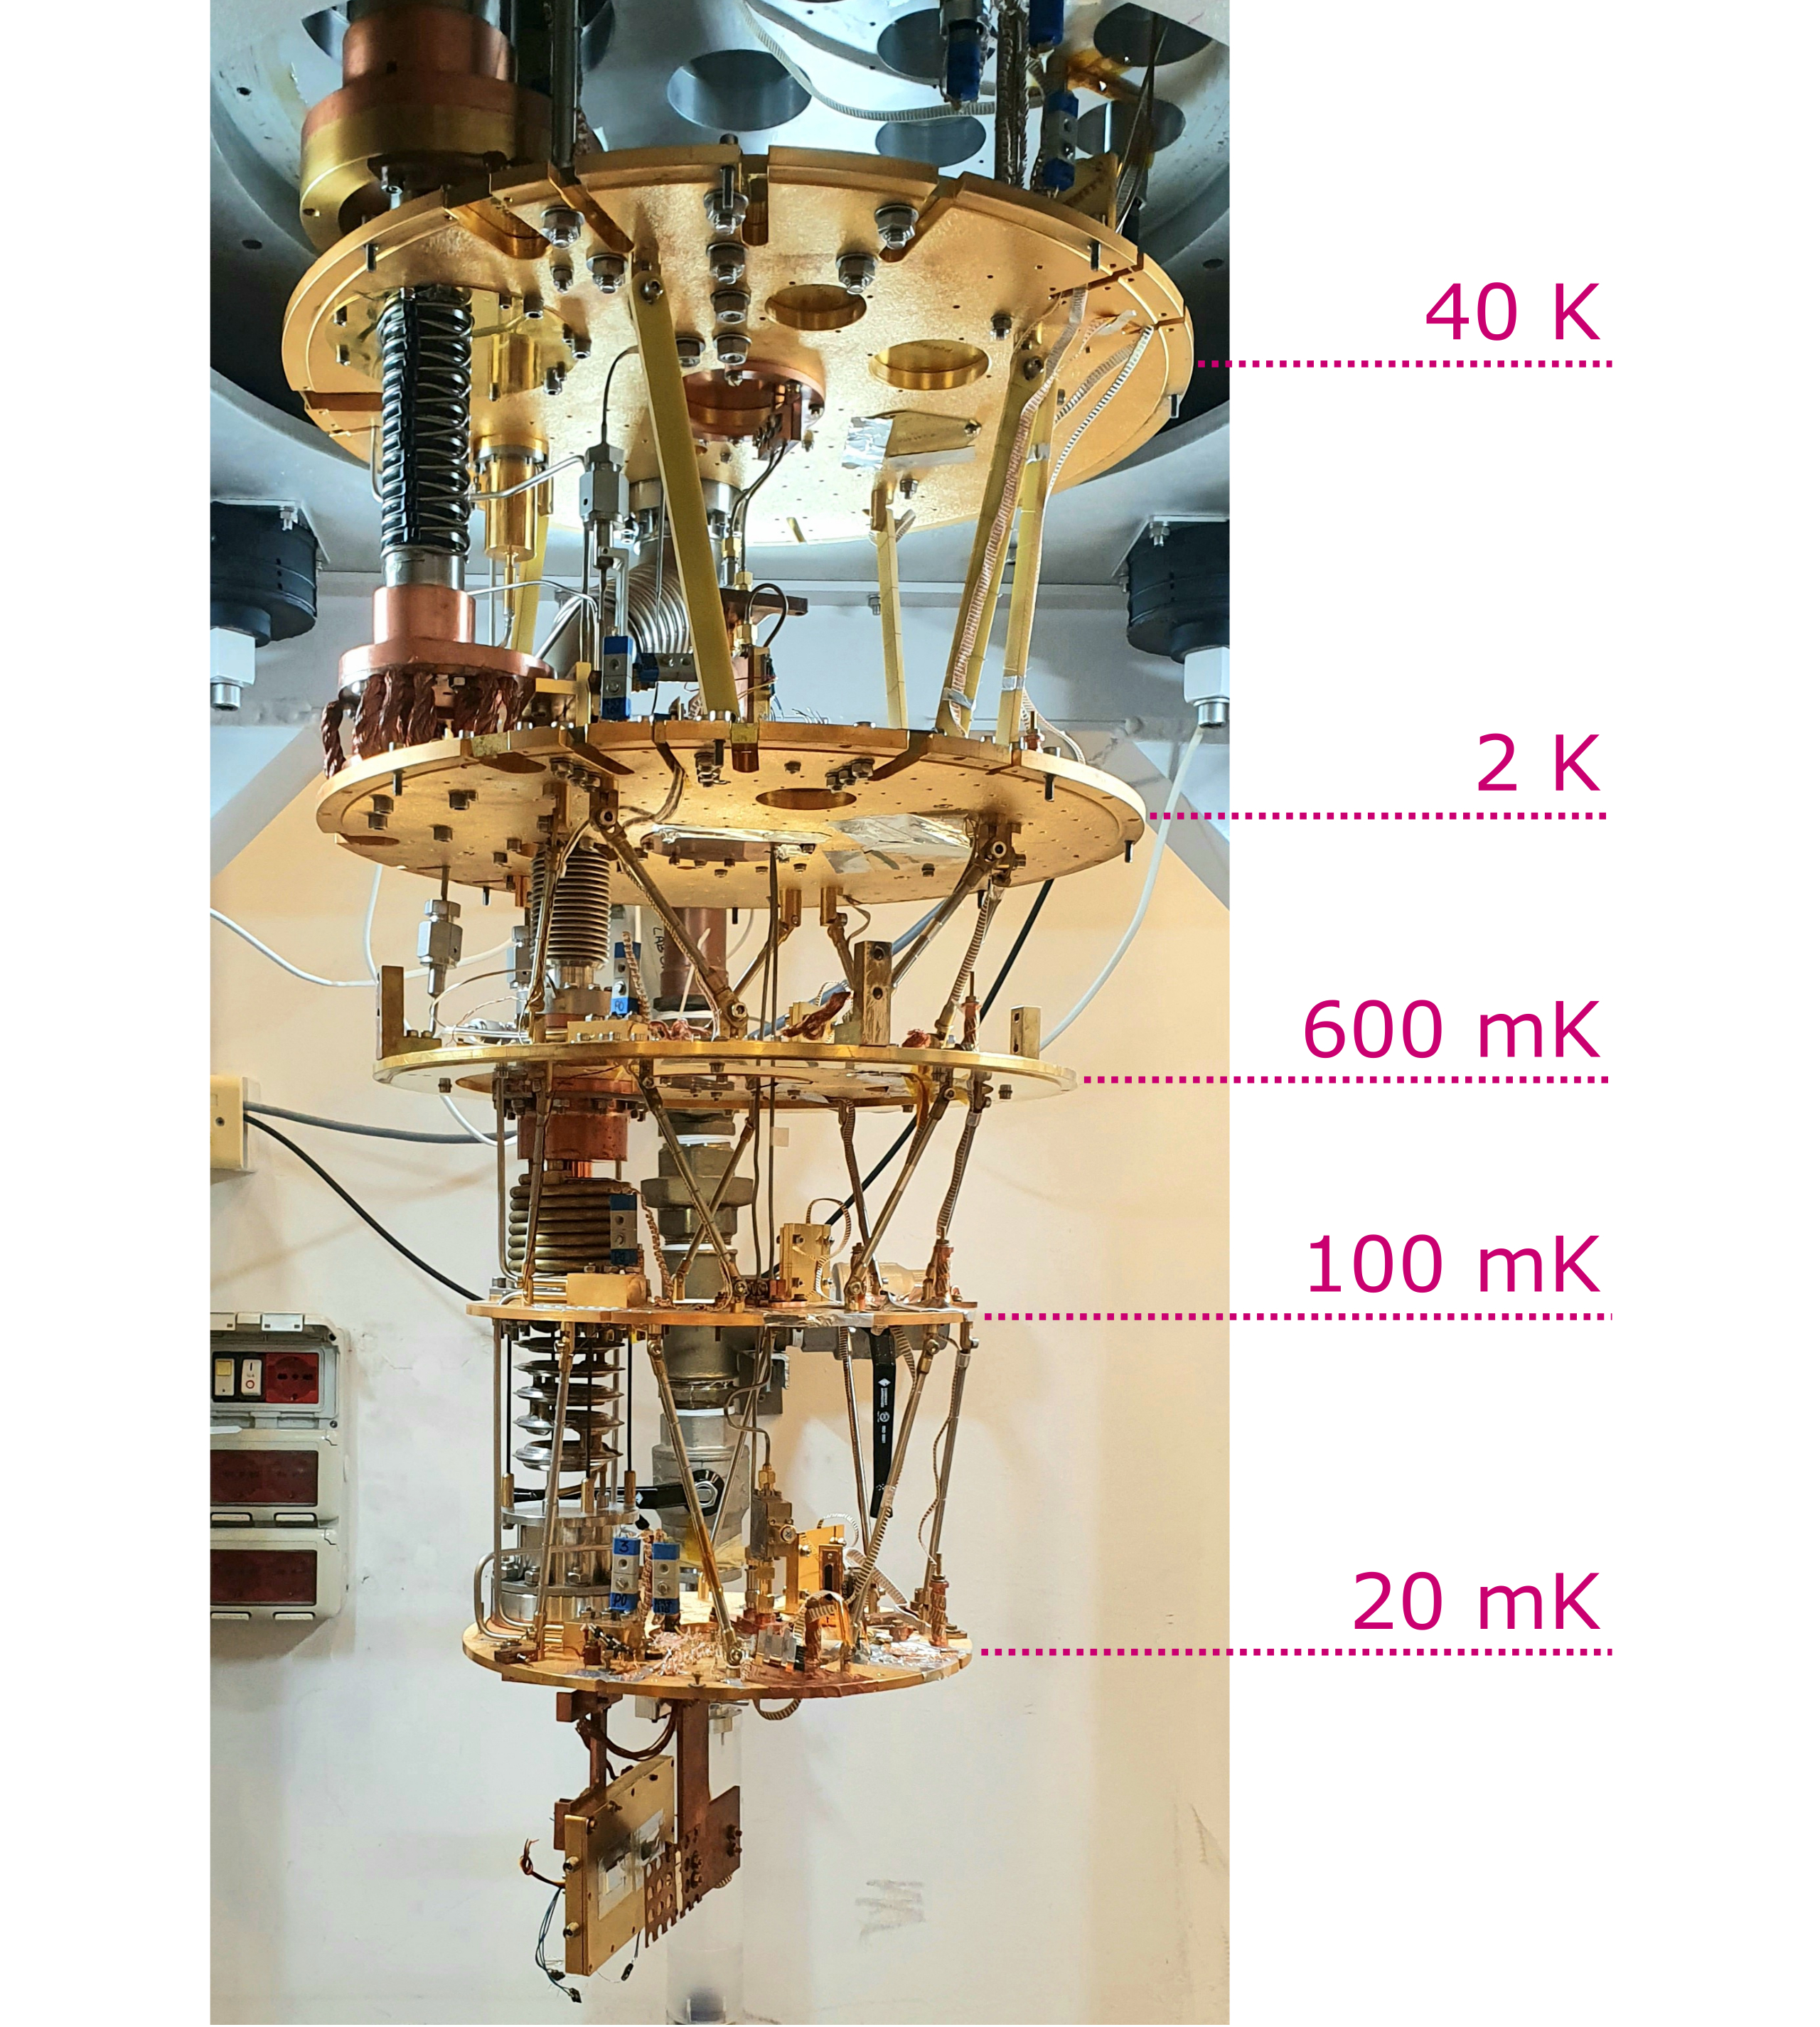
\includegraphics[width=\linewidth]{figures/ch1/cryo.jpg}
\caption{}
\end{subfigure}
\hfill
\begin{subfigure}[b]{0.45\linewidth}
    \includegraphics[width=\linewidth]{figures/ch1/holder.jpg}
\caption{}
\end{subfigure}
\caption{The dilution refrigerator used by Holmes (a). Close-up of the detectors holder mounted to the mixing
chamber's plate (b).} 
\label{fig:cryo}
\end{figure}
To achieve the required vacuum level of around $10^{-6}$ mbar, a diaphragm pump and a turbomolecular pump are employed. A series of thermal shields made of aluminum and copper are securely fastened to different plates to prevent thermal radiation from transferring between the various temperature stages.
Since the rf-SQUIDs are highly sensitive magnetometers, a substantial magnetic shield is mounted and connected to the
second-stage 2K plate. The detectors holder is attached to a copper plate under the coldest
refrigeration stage, the mixing chamber plate, and further thermalized with copper braids. 


The microwave probe tones used for the multiplexed readout must travel from the warm 300K electronics to the 60mK cold
stage where the $\mu$MUX chip is located. Copper-nickel coaxial cables are used for this purpose between 300K and 4K.
After a 20 dB attenuation at 2K to match thermal noise levels, the signal is transmitted
through stainless steel cables and undergoes another 20 dB attenuation before entering the detetors holder. Upon exiting
the box, it passes through a circulator that shields the detectors from the noise generated by the following amplification stage, which uses a low-noise High Electron Mobility
Transistor amplifier (HEMT) placed on the 2K plate. In this stage,
connection is established using superconducting Nb coaxial cables to avoid signal dissipation and ensure minimal thermal
conductance, while the amplifier models (LNF - LNC48A) offers optimal noise performance in the working frequency range
of 4-8 GHz. 
The voltage ramp signal required for $\mu$MUX multiplexing demodulation and the voltage bias for the detectors are transmitted using Nb-Ti twisted pairs, which are themselves thermally linked to each temperature stage through contact, forming a ribbon on a small copper rod fastened to each plate.
Various heaters and thermometers are distributed across the different plates, allowing for comprehensive monitoring and control of the cryostat's behavior during measurements.



\subsection{Warm electronics setup}
The system for the multiplexed readout of the detectors is built upon electronics initially developed for the readout of
Microwave Kinetic Inductance Detectors (MKIDs). The probe tones are generated in the Mhz range, then up-converted to Ghz with an IQ mixer and read using an heterodyne readout scheme. The main components of
this setup are:
\begin{description}
\item[ROACH2:] Denotes the 2nd-generation Reconfigurable Open Architecture Computing Hardware (ROACH2) platform.
This system consists of a digital board housing a Xilinx Virtex 5.1 FPGA for signal processing and a PowerPC
440EPx for slow control, which are paired with a peripheral DAC/ADC board hosting two DACs (1000 MS/s, 16 bit, 75 dBc of NSD) and two ADCs (550 MS/s, 12 bits, 64 dB of SNR) for generating and acquiring in-phase and quadrature signals.
Sinusoidal probe tones, one for each microresonator to be readout, are generated by the DACs using a Direct Digital
Synthesizer (DDS) and an external clock source, which is provided by a Valon synthesizer, resulting in I and Q
components with a baseband frequency range of 10-512 MHz.
Moreover, the FPGA firmware implements some fundamental processing algorithms such as the channelization of
different frequencies of the signal and the sampling of the flux ramp modulation through Fourier measurements.
The acquired data are transmitted from the ROACH2 board to a workstation computer via a 10 Gb/s Ethernet connection.

\item[IQ mixer] 
An IQ mixer is a fundamental device used in radio frequency and microwave
systems. It combines two input signals, typically a local oscillator (LO) signal and a radio frequency (RF) signal, to
generate two output signals: the in-phase (I) and quadrature (Q) components. These components represent the real
and imaginary parts of a complex signal oscillating with a frequency given by the difference bewteen that of the RF and
the LO. Alternatively, a low frequency signal with given I and Q can be modulated to the RF band by mixing it with
the LO. The heterodyne readout scheme employs both of these techniques. Up-conversion to the RF frequency range (4-8 GHz)
suitable for the multiplexer chip is achieved by mixing the I and Q generated by the ROACH2 with the LO. The IQ mixer
used by Holmes is a PXIe Hybrid with a design customized for the 4-8 GHz frequency range, matching the HEMT
bandwidth for reduced signal loss.
The modulated output tones are amplified with a gain of 26 dB and then down-converted from RF to baseband using the same
board and LO signal. The output signals I and Q are then amplified again to fully utilize the dynamic range of the two ADCs.

\item[Bias and flux ramp:]
These components play critical roles in signal reconstruction and detector stability.
The voltage bias employs a very stable power supply constructed from two large batteries, providing
stability up to ppm/$^\circ$C for the operating voltage of $\sim 500mV$.
The ramp is created by a standard signal generator. To minimize disturbances, such as ground loops and electromagnetic
interference, a custom coupling transformer is used between the signal generator and the input of the cryostat.

\end{description}
The electronics configuration is shown in Fig \ref{fig:warmelrctronics}. To synchronize all the components (ADCs, DACs,
FPGAs, and LOs), a common external clock is provided by a 10 MHz rubidium frequency standard. In the current
configuration, the ROACH2, IQ mixers, HEMT and external amplifiers are doubled to allow for the simultaneous readout of up to 64
detetctors.

\begin{figure}[t]
  \centering
  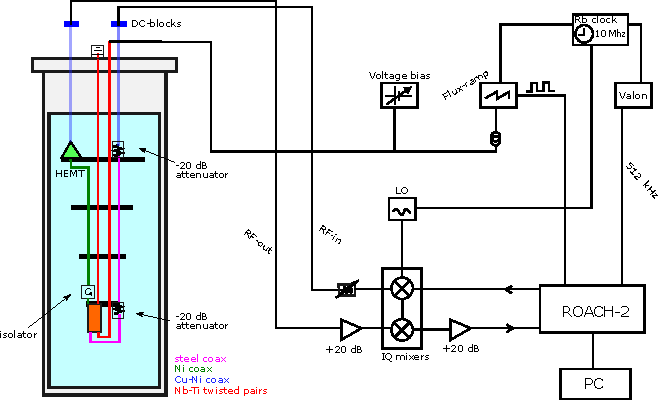
\includegraphics[width=0.74\textwidth]{figures/ch1/warmcircuit.pdf}
  \caption{Electronics circuit for the Holmes experiment. The current setup empoys two ROACH2 and four IQ mixers to read
  up to 64 detetctors at the same time.}
  \label{fig:warmelrctronics}
\end{figure}

\subsection{First $^{163}$ Ho implantation}
In its current configuration, shown in Fig \ref{fig:implanter}, the implanter consists of a Danfysik Model 921 A sputter ion
source, a 1 T magnetic dipole mass analyzer, a slit for geometrical selection, a Faraday cup for beam diagnostics and a target holder. 

In the ion source, four hot tantalum wires emit electrons through thermionic emission. These electrons are then
accelerated by a discharge potential and traverse an argon gas, creating a plasma. This plasma is then accelerated by a sputtering potential towards an electrode disk where a suitable Holmium target is situated.
The sputter target consists of a Zr/Bi (98\%/2\%) sintered matrix on which a 
$^{163}$Ho(NO$_3$)$_3$ solution is dripped to obtain an uniform distribution.
The argon ions sputter off Holmium and the other materials comprising the target. Once the Holmium atoms are
ionized by interaction with the plasma, they are accelerated by an extraction voltage ranging from 30 to 50 kV and exit the source in an ion beam, alongside the argon ions and other contaminants present on the target and in the chamber.
Subsequently, the ions pass through a small magnet capable of bending the beam along the z-axis for alignment before
entering the magnetic selector, which separates and isolates $^{163}$Ho from
other contaminants. The primary contaminant is $^{166m}$Ho, a byproduct of the $^{163}$Ho production process that decays with a
low-energy beta spectrum.
The purified Ho beam is then directed through a slit, trimming the beam tails and further reducing the likelihood of
other contaminants reaching the detectors, and Faraday cup, which measures the beam's current. Finally, the beam
reaches the TES arrays, which are mounted onto a target holder that can be moved vertically.

\begin{figure}[t]
    \begin{subfigure}[b]{0.44\linewidth}
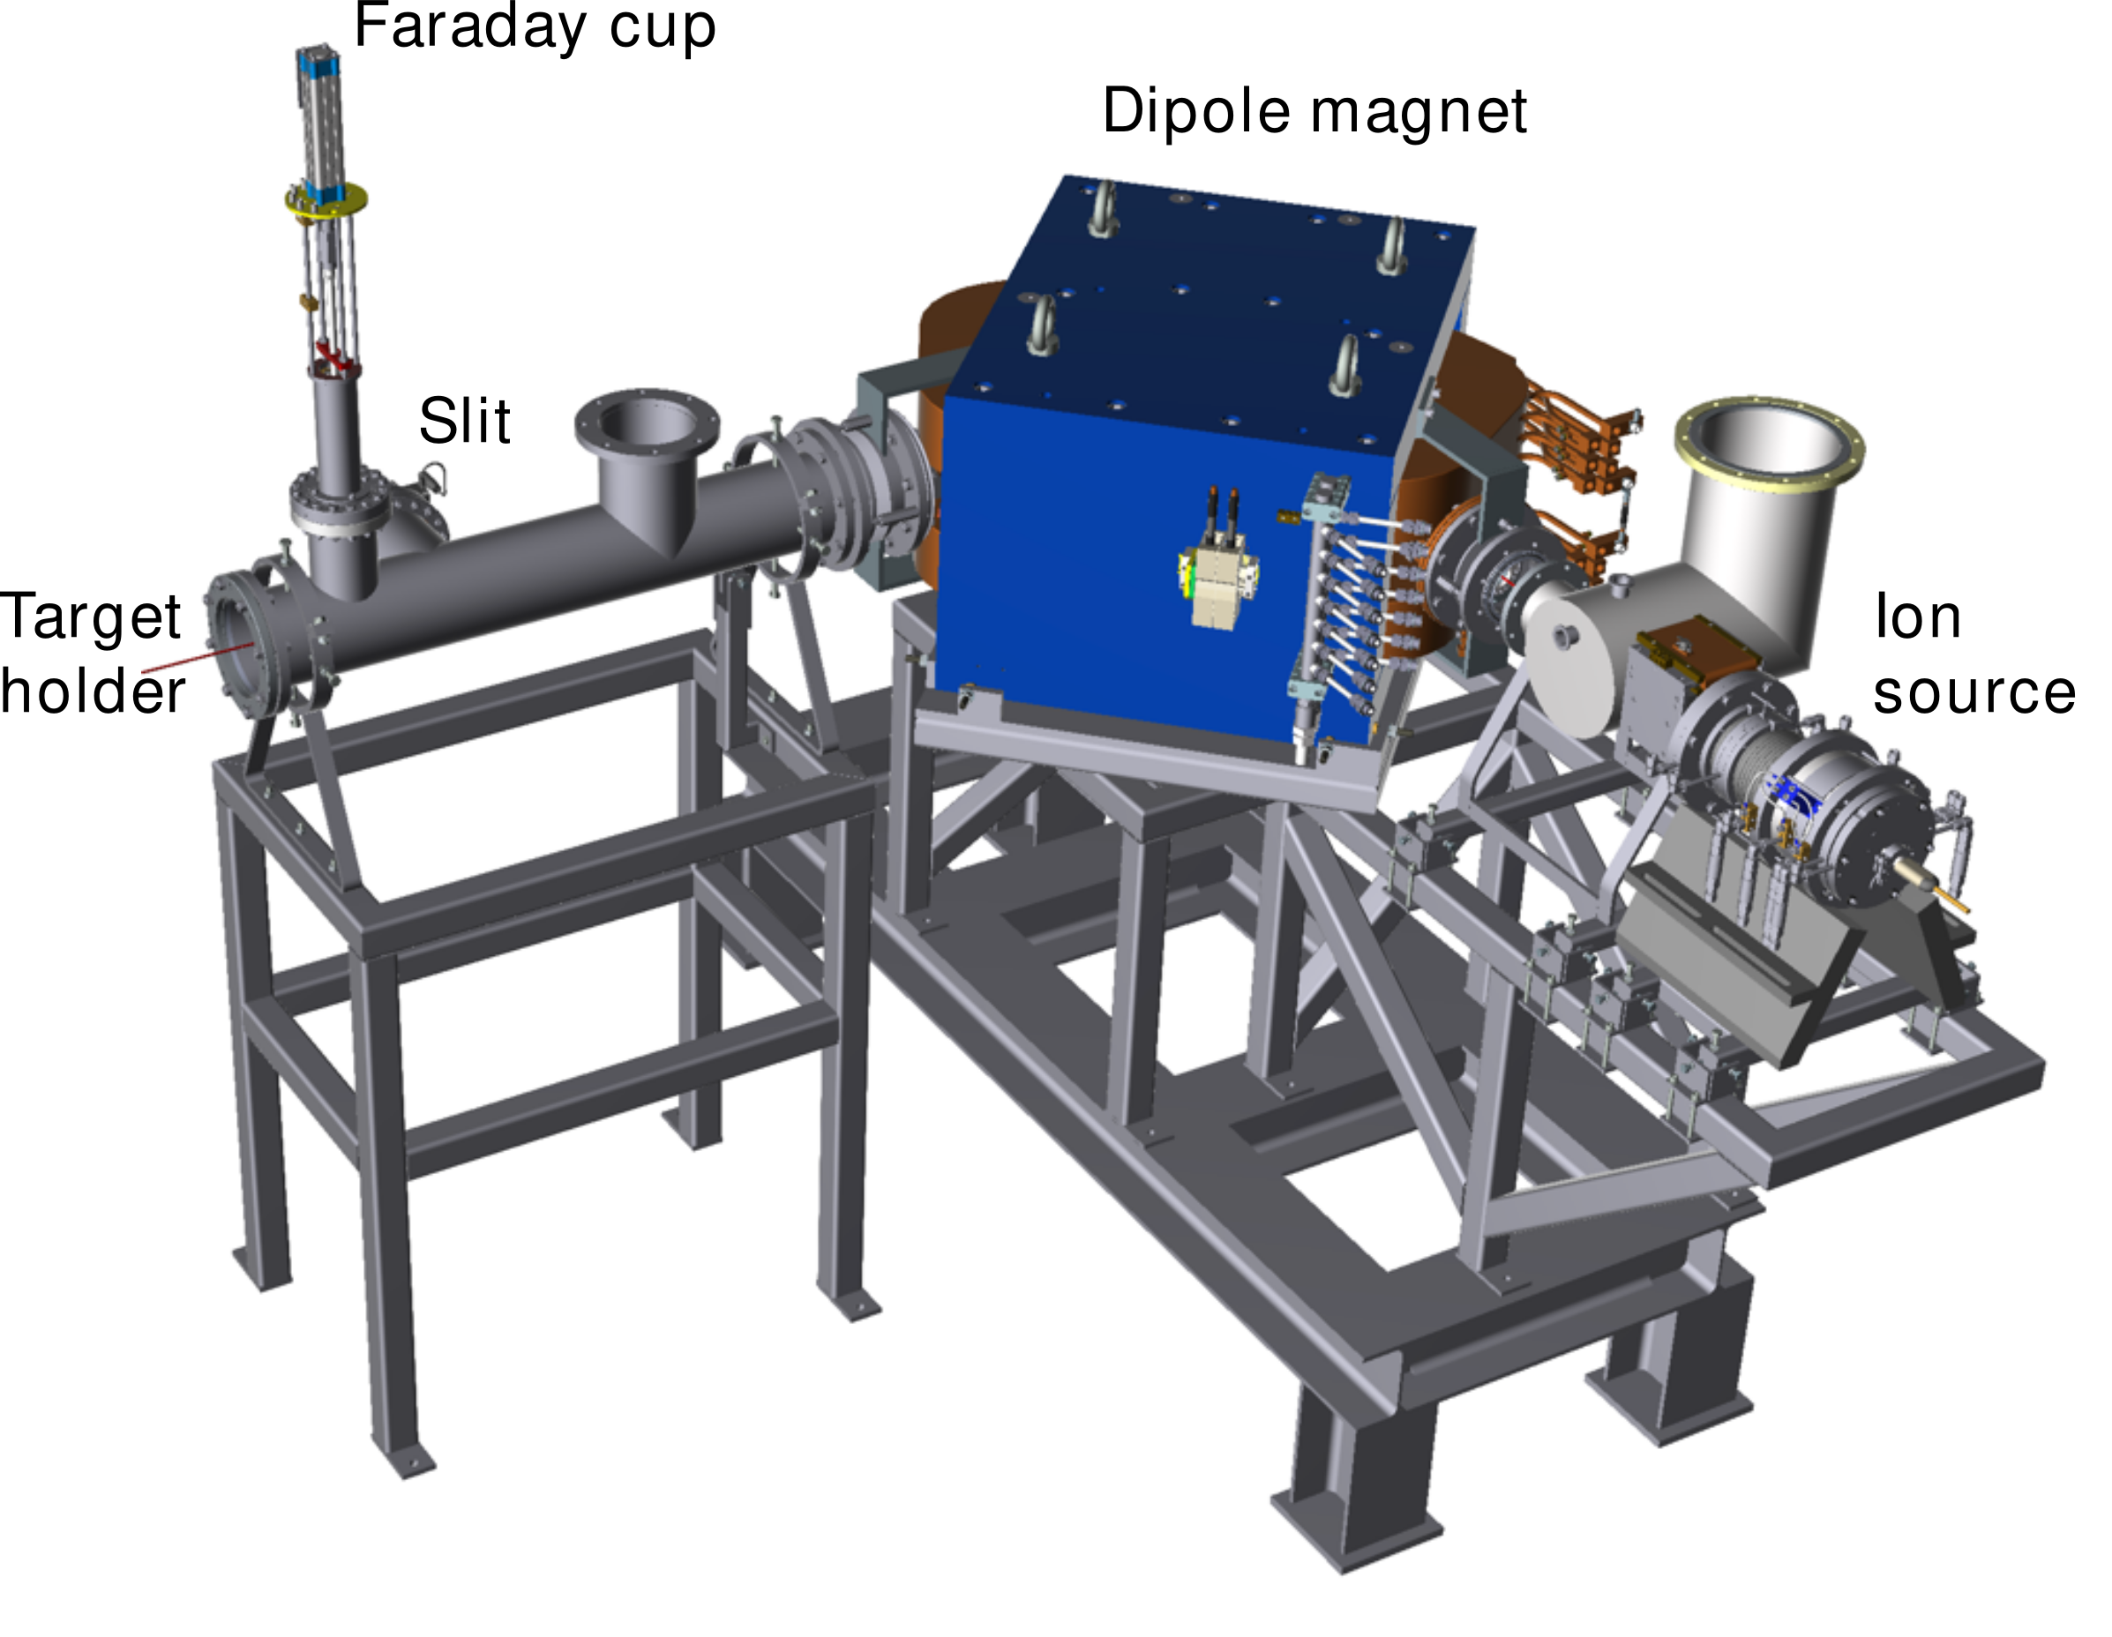
\includegraphics[width=\linewidth]{figures/ch1/implanter.pdf}
\caption{}
\end{subfigure}
\hfill
\begin{subfigure}[b]{0.4\linewidth}
    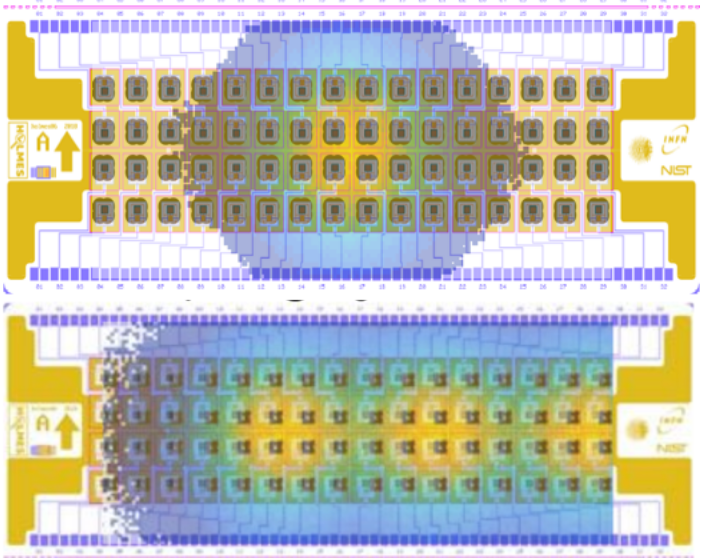
\includegraphics[width=\linewidth]{figures/ch1/implantationMC.png}
\caption{}
\end{subfigure}
\caption{Custom ion implanter used to embed $^{163}$Ho in the gold absorbers of the detector arrays (a). Monte Carlo
simulations of the expected implanted Ho distributions over the detectors for the first measurement campaing of Holmes
(b).}  
\label{fig:implanter}
\end{figure}
Looking ahead, there are plans to enhance the capabilities of the implanter. This includes the incorporation of an
electrostatic triplet and magnetic XY scanning to provide greater beam focus and control over its direction.
Simultaneously, the target chamber described in Sec \ref{sec:fabrication} will be added to the end of the apparatus, enabling Holmium implantation while
depositing gold on the absorbers. This dual function aims to achieve higher activity levels and embed the radioactive source in the full volume of the absorber rather than in a single layer.

After a series of calibration and characterization runs with $^{165}$Ho \cite{Hoimplant}, the custom ion implanter has
been utilized with $^{163}$Ho for the first time. The current implantation efficiency is anticipated to be approximately
0.2\%. Despite this small value, it remains suitable for a low-dose implantation.
Two sets of 64-TES arrays were implanted, each following a distinct pattern as shown in the simulations of Fig
\ref{fig:implanter}. The first array was targeted at a single
central spot to evaluate the beam profile and assess the impact of Holmium on detector properties. The central pixel is expected to exhibit an activity of approximately 3 Bq.
In contrast, the second array was implanted in three spots, with the aim of achieving an approximately uniform activity
of 1 Bq across all detectors. These two resulting detector arrays are the fundamental components in the first measurement campaign of the Holmes project.
